%Page Setup to University standards  ----------------------------------------------
\documentclass[12pt,oneside,listof=totoc,paper=a4,headings=small]{scrbook}
\renewcommand{\baselinestretch}{1.3} 
\usepackage[utf8]{inputenc}
\usepackage[a4paper, left=35mm,right=15mm,top=30mm,bottom=25mm]{geometry} 
%  ----------------------------------------------

%Titlepage credentials  ----------------------------------------------
\title{Evolutionary Computational Modeling in a 3D Physics Environment}
\author{David Richter}
\date{October 2018}
% ----------------------------------------------

\usepackage{mathptmx}   %font
\usepackage{subcaption} %Table of images

\usepackage{natbib}
\usepackage{graphicx}
\usepackage[dvipsnames]{xcolor}

\usepackage{float} %Make images appear where they are in code

\newcommand{\source}[1]{\caption*{Source: {#1}} } %For giving source to images


\usepackage{hyperref} %Reference a URL


% Header ------------------------------------------------------------
\usepackage[headsepline,manualmark]{scrlayer-scrpage}
\clearpairofpagestyles
\ohead{\pagemark}
\ihead{\headmark}
\automark{chapter}
\pagestyle{scrheadings}
\renewcommand*\chapterpagestyle{scrheadings}


%For Code displays ----------------------------------------------
\usepackage{listings}
\usepackage{color}

\lstset{basicstyle=\footnotesize\ttfamily,breaklines=true}
\lstset{framextopmargin=50pt,frame=bottomline}

\definecolor{codegreen}{rgb}{0,0.6,0}
\definecolor{codegray}{rgb}{0.5,0.5,0.5}
\definecolor{codepurple}{rgb}{0.58,0,0.82}
\definecolor{backcolour}{rgb}{0.95,0.95,0.92}
 
\lstdefinestyle{mystyle}{
    backgroundcolor=\color{backcolour},   
    commentstyle=\color{codegreen},
    keywordstyle=\color{magenta},
    numberstyle=\tiny\color{codegray},
    stringstyle=\color{codepurple},
    basicstyle=\footnotesize,
    breakatwhitespace=false,         
    breaklines=true,                 
    captionpos=b,                    
    keepspaces=true,                 
    numbers=left,                    
    numbersep=5pt,                  
    showspaces=false,                
    showstringspaces=false,
    showtabs=false,                  
    tabsize=2
}
\lstset{style=mystyle}
% ----------------------------------------------


\begin{document}

%\maketitle
\frontmatter


\thispagestyle{empty}
\vspace*{-20mm}

\begin{center}

\includegraphics[width=0.5\textwidth]{images/2000px-Logo_Hochschule_Kempten.png}
\end{center}

\vspace*{1cm}
% Alle Elemente sollen zentriert sein
\begin{center}
% Art der Arbeit => (Bachelorarbeit ,Diplomarbeit, Masterarbeit, Studienarbeit)
{\Large \textbf{Bachelor's Thesis}}\\
\vspace*{0.5cm}
{\large Computer Science (Bachelor)\\[1mm]}
{\large Kempten University\\[1mm]}
\vspace{0.5cm}
% Titel der Arbeit
{\Large \bfseries Evolutionary Computational Modeling\\ in a 3D Physics Environment\\}
\vspace{1cm}
% Name des/der Autors/Autoren
{\large David Jona Richter}\\[40mm]
\end{center}
\vfill

\begin{center}
\parbox{120mm}{
\begin{tabbing}
Instructor/Corrector in Kempten \hspace{1.45cm} \= Prof. Dr. J. Staudacher\\
Submission Deadline                        \> March 14th 2019\\
Department in Kempten                  \> Faculty of Computer Science\\
Lab at MSU \> Hintze Lab\\
Instructor at MSU                   \>Prof. Dr. A. Hintze\\
Author                              \> David Richter \\

Author's Contact Data               \> david.j.richter@stud.hs-kempten.de
\end{tabbing}
}
\end{center}

\newpage
\vspace*{0.5cm}
\begin{center}
{\Large \color{OliveGreen} \underline {MICHIGAN STATE UNIVERSITY}}
\end{center}
\begin{center}
 This Thesis was written to complete my Bachelor of Science in Computer Science at Kempten University. The Research for this work was conducted at Hintze Lab at Michigan State University.
\end{center}

\newpage

\vspace*{1cm}

\begin{center}
    \textbf{Abstract}
\end{center}

\vspace*{1cm}

\noindent
This paper contains the process of having implemented DART (Dynamic Animation and Robotics Toolkit), an open source physics engine, usually used mainly for robotics, into MABE (Modular Agent-Based Evolution platform), a tool to evolve and analyze digital brains, using C++. This added much desired complexity to the system which allows the Hintze Lab to further research evolution and added new ways in which they can do so. Furthermore, the resulting software package was used to run a series of experiments in this work, which will then be analyzed and compared.


\tableofcontents
\listoffigures
\lstlistoflistings
\listoftables

\clearpage
\mainmatter
\setcounter{page}{1}

\chapter{Introduction}
\section{How to study evolution?}
The famous evolutionary biologists Dobzhansky once said that ``Nothing in biology makes sense unless seen in the light of evolution''~\cite{dobzhansky2013nothing}. This quote stresses the importance to understand evolution and explains why so much research is carried out in this field. Evolution not only explains the origin of species~\cite{darwin2004origin} but also the change that happened to life on earth as a whole. However, studying evolution by observing real live organisms and their changes and mutations is inconvenient to say the least, since the process is really slow and takes a long time to develop. It is also difficult to have control over what is happening since so many variables have effect on the organisms. There are only few examples, like the long term evolution experiment carried out on 60.000 generations of \textit{E. coli}~\cite{lenski2003evolutionary}, which allow for the study of evolutionary processes under laboratory conditions. Doing such an experiment with vertebrates for example, is not only too expensive, but nobody would have the time to wait for even a few generations (say a 100) to pass. Fortunately, evolution as a process is substrate independent, and is not necessarily bound to living organisms.
\subsection{What is evolution?}
\begin{figure}[h!]
\centering
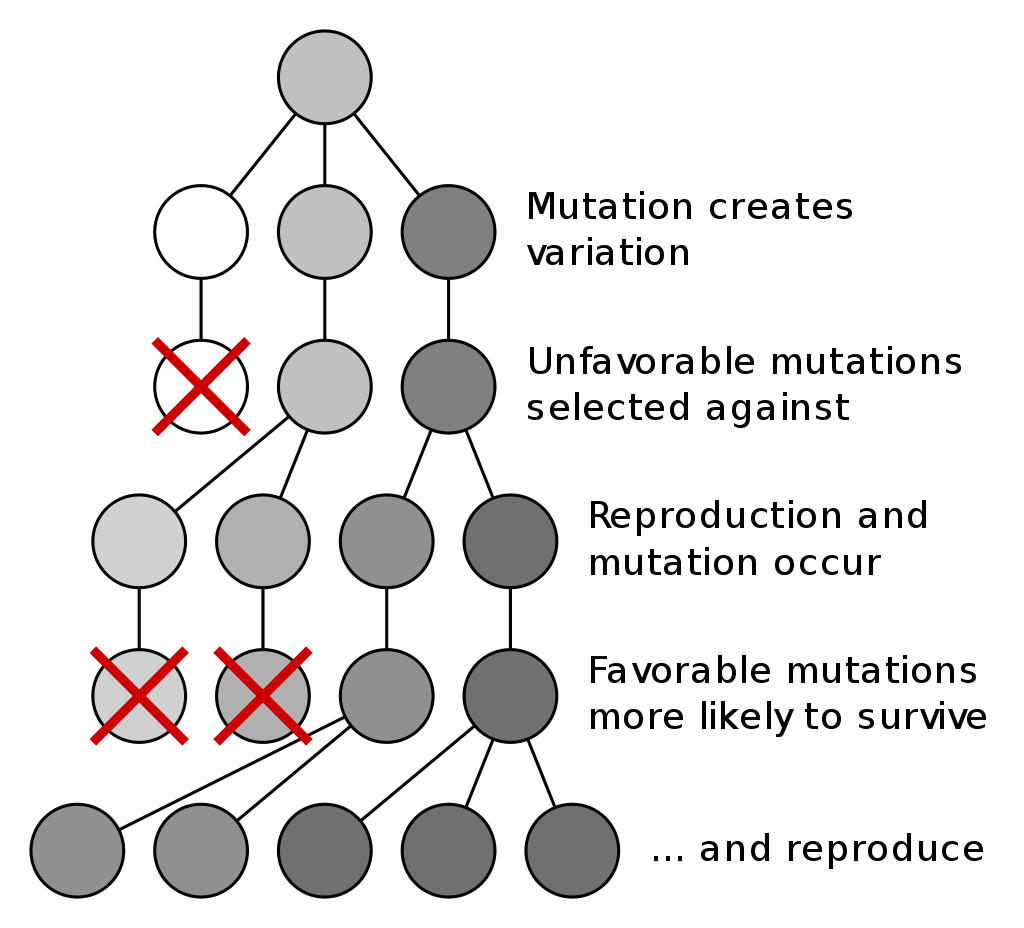
\includegraphics[width=0.75\textwidth,height=0.75\textheight,keepaspectratio]{images/1024px-Mutation_and_selection_diagram.png}
\caption{A diagram that shows inheritance, variation, and selection being applied.~\cite{evolDiagram}}
\label{fig:evolution}
\end{figure}
%https://en.wikipedia.org/wiki/Evolution#/media/File:Mutation_and_selection_diagram.svg
We talk about evolution, but what really is it?  And how does it actually work?
Evolution is the theory that explains the ``Artenfrage''~\cite{darwin2004origin}, that is: why is Nature so diverse, while each species is so distinctly different? Darwin proposed a simple mechanism comprised of three necessary and independent principles~\cite{huxley1942evolution}: Inheritance, variation and natural selection (see Figure \ref{fig:evolution}). 
Since this work deals with a computational system, and the term ``natural'' is already questionable, from now on the term selection is used instead of ``natural selection''.

Evolution started the moment self-replicators appeared on earth. This is important, since evolution does not explain the origin of life, but instead explains what happens to life once it appears. As the word self-replicator implies, they are entities that have the ability to create copies of themselves. 

Since evolution is inheritance, variation, and selection, a computer model must define these three principles. While inheritance is typically as simple as copying memory, the other two are of more importance. Selection is a mechanism that chooses which organisms are allowed to make offspring. This can happen in many ways. If selection would be random, each organism would have the same chance to make offspring. The random selection method is thus used as a way to test if other selection methods work.

In more detail \textbf{Inheritance} now describes the fact that from generation to generation, the offspring a self-replicator creates, inherits the traits of its parent: self-replicators create exact copies of themselves. In actual organisms, this could be as irrelevant as hair color, it could be the blood type, it could be a disability and much more. Basically all traits that are being stored in one's DNA are subject to inheritance. Inheritance does not just occur generation to generation, but can also appear over greater lengths. That means, that if somebody's great-grandmother had red hair, even if for two generations there has not been anybody that was born with it, the genes could still lie within the DNA and that the expression of red hair could resurface in future generations again.
Technically, inheritance explains why we have more than a single life form but multiple copies of it.


\newpage
\textbf{Variation} as the second principle is needed to explain the diversity around us, instead of every organism being a ``clone'' of a self-replicator. It is the reason that humans look different, have different shapes and sizes. Without variation we would all essentially be identical. Variation is in nature synonymous with mutations and recombination and as such is created when offspring is made. In asexual organism's mutations lead to the changes in the offspring. In sexual organisms it is mutations and recombination of the parental genomes that lead to variations in offspring. Since inheritance is already a requirement for evolution, the variation created is propagated to future generations, and can interact with future mutations. This compounding effect of mutations is one reason why evolution is such a powerful search method. One early example of variation being observed and recorded are the so called ''Darwin's finches`` (see Figure \ref{fig:darwinsfinches}). The term has been coined by Percy Lowe in 1936 and David Lack in 1947. Darwin's finches are also known as Galápagos finches, because they can be found on the variouos islands in that region. They are group of passerine bird's, about 15 species big. Since their beaks are so distinctly different in form and function they are commonly used to explain and display variation within a species. 

\begin{figure}[h!]
\centering
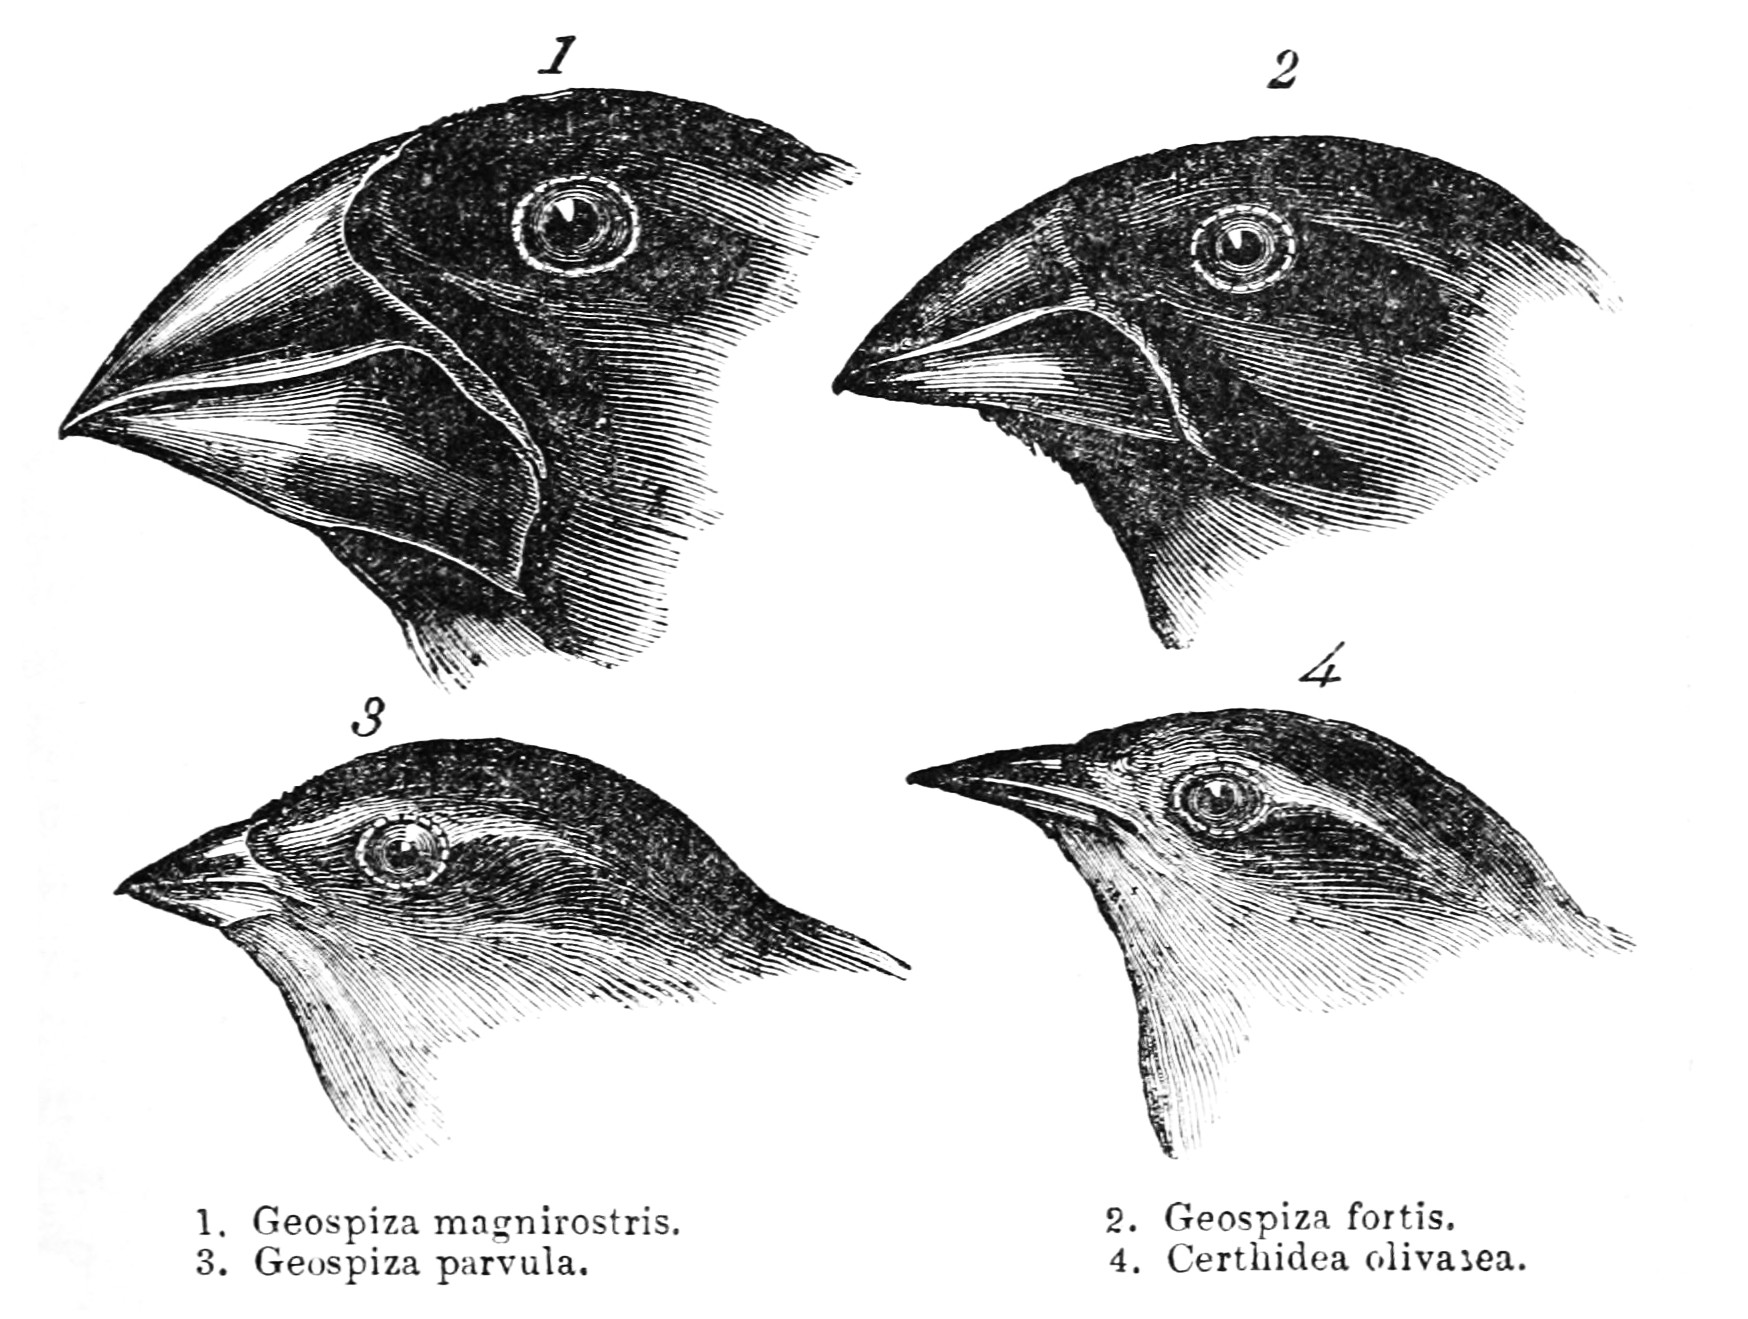
\includegraphics[width=0.6\textwidth,height=0.6\textheight,keepaspectratio]{images/variation_Darwin's_finches_by_Gould.jpg}
\caption{An image that shows the various different beaks that are known as Darwin's finches~\cite{DarwinsFinches}}
\label{fig:darwinsfinches}
\end{figure}
%https://upload.wikimedia.org/wikipedia/commons/a/ae/Darwin%27s_finches_by_Gould.jpg

Inheritance and variation alone would create a planet populated with many different organisms, all randomly different from each other. However, we observe discrete species, with most of their individuals sharing many traits, while also being distinctly different from other species. A pure random process would not explain speciation and the type of complexity we observe.

\newpage
\textbf{Selection}, as the last necessary factor, explains this type of structured outcome of evolution, while also explaining why over evolutionary time organisms keep adapting (becoming better over generations). Selection results from organisms having different reproductive success. An organisms that carries traits that make it replicate faster will create more copies (with mutations) than an organism without that trait. Competition between these organisms about resources will lead to the extinction of the organism that is replicating slower. Selection describes this phenomenon, and explains that organism that replicate faster are preferentially selected over those that replicate slower. Darwin called this phenomenon ``survival of the fittest'', where fitness is an abstract concept quantifying replication success. Fitter organisms found a way to replicate faster.

\section{Why is evolution difficult to observe?}
To understand why evolution is almost impossible to observe, study, analyze, and research in real live, we have to take a quick look at how and why evolution works.
In sexual reproduction, the offspring carries parts of the fathers and mothers DNA and therefore obtains traits from either one of them. Some of them might be beneficiary, other might not be or might even turn out to be a disadvantage, bad eyesight for example. If we look at a world before our time, in which we are not yet living in relative luxury and where negative traits, like the above mentioned eyesight, are easily correctable, such traits could greatly limit ones life expectancy and their performance during that time, which could have bad influence on natural selection.
Also, random mutations which could also have positive or negative effect on an organism can occur, six toes on ones feet for example. Again, these will affect fitness and therefore have an effect on the selection process, and if it turns out to be favorable it could lead to a shift in the population.
All of this take millions of years. We humans for example already live as \textit{Homo sapiens} for at least 200.000 years~\cite{mcdougall2005stratigraphic}, which is obviously way to long for any study to follow in the slightest. For research purposes we either need to speed up time and evolution itself, find somebody that can grow over a million years old, or model the process and do research that way.

\newpage
\section{The difference between simulating and modeling evolution}

Simulation and modeling, are often uses synonomously. They often describe a similar process and are thus confused, even though their entail an important technical difference.

Simulation is originally meant to describe the process of writing a program or setting up an experiment that is meant to make the observer believe he is watching reality. It is supposed to ``fake'' reality. Imagine the original mechanical Turk (see Figure \ref{fig:mechanica_turk}). A machine that supposedly played chess using an mechanical automation. However, the machine contained a human (small grown turk male - hence the name). The machine was build to make the audience believe there is a mechanical intelligence at work, even though it wasn't. It simulated a chess computer. 

\begin{figure}[h!]
\centering
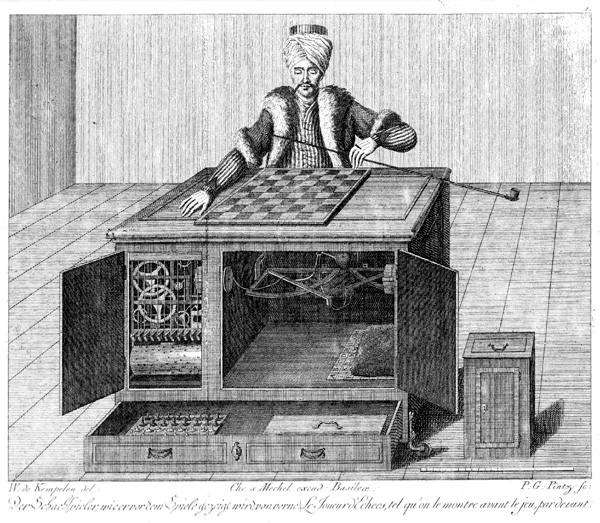
\includegraphics[width=0.75\textwidth,height=0.75\textheight,keepaspectratio]{images/Tuerkischer_schachspieler_windisch4.jpg}
\caption{A drawing of the Mechanical Turk, a device that pretended to play chess animatedly.~\cite{mechTurk}}
\label{fig:mechanica_turk}
\end{figure}
%https://en.wikipedia.org/wiki/The_Turk

Modeling on the other hand is meant to be real. To follow reality not just in its visualization, but also in the processes behind it and leading up to it. Modeling is supposed to not just look real but also behave like reality even after leaving the scripted environment to which simulations are limited. An actual chess computer indeed plays chess using electronic computation, and is not ``faking'' intelligence. It actually plays chess. In the context of evolutionary modeling, this contrast is more obvious. Instead of pretending that something evolves, computer code or strings of virtual DNA actually experience inheritance, selection, and variation and thus do evolve. Evolution inside a model, if done properly, becomes an instance of evolution and not a simulation ~\cite{Pennock:2007iy}. This is what MABE~\cite{bohm2017mabe,MABE2016} is striving for, to create and experience real evolution and study it's results.

As a consequence, we can use computational evolutionary models to study evolutionary principles directly. 

\chapter{Computational models of Evolution}
Because evolution is substrate independent, we can study evolution in a different context altogether. Using computational models seems to be a cheap, quick, and reliable alternative. In particular, since computational models in evolution are not just ``simulations'', but in fact instances of evolution themselves ~\cite{Pennock:2007iy}.

To create such a model we need to implement inheritance, variation, and natural selection into it. Inheritance is being handled by creating genomes, which can be thought of as long strings of letters and numbers, that can be used to be projected onto a given attribute within our model, or simply copying the agent itself. Variation is being taken care of with random mutations that can happen each time offspring is being produced. Selection must be defined by a fitness function that varies from application to application. This is the way in which it is already encoded in  genetic algorithms.

Among the many computational tools to study evolution (AVIDA~\cite{adami1994evolutionary}, EAVOL~\cite{knibbe2007long}, EaLib~\cite{dknoester2016ealib}, NEAT~\cite{stanley2002evolving}, HyperNEAT~\cite{gauci2007generating}), %citations
we also find MABE: the Modular Agent-Based Evolution platform developed by the Hintze Lab~\cite{MABE2016,bohm2017mabe}. This MABE platform is built in a modular fashion. These modules can be modified or new ones can be added. This makes MABE a convenient tool to create new experiments, reuse code from others, and to extend previous work. 
Sharing work, results, and entire experiments with MABE is very easy, because of its modular architecture. The plug and play principle is a big leap into the right direction. MABE is making the process a lot less tedious, even combining projects is no problem anymore, since again, modules simplify the process immensely.

%----- Experiemente können kombiniert werden und sachen getauscht werden mit anderen leuten

\newpage
\section{MABE}
\subsection{MABE Modules}
MABE is made up of multiple modules (see Figure \ref{fig:MABE_Modules}) that are interchangeable with other components that fit the modules requirements, brains can be swapped with other brains, for example. The modules are as follows: 
\begin{figure}[h!]
\centering
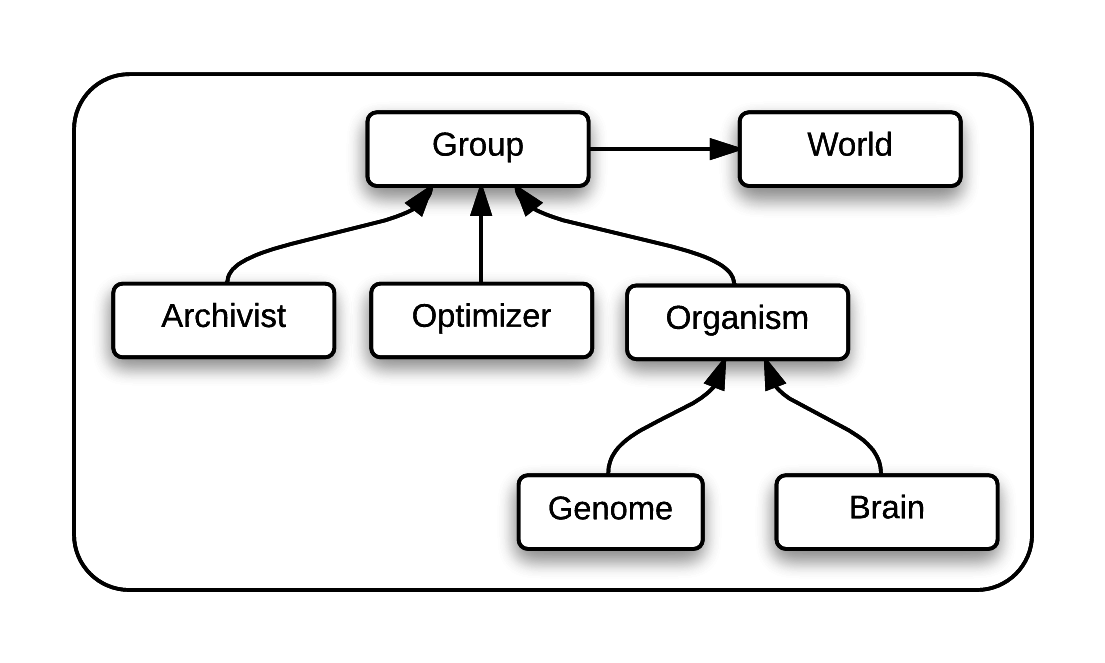
\includegraphics[width=0.75\textwidth,height=0.75\textheight,keepaspectratio]{images/MABE_Overview.png}
\caption{A diagram of the modules in MABE and how they relate to one another.~\cite{mabeModuleChart}}
\label{fig:MABE_Modules}
\end{figure}
%https://raw.githubusercontent.com/wiki/Hintze Lab/MABE/images/MABE_Overview.png

\subsubsection{Brains}
Brains in MABE process inputs to then give outputs which are part of a continuous list of values. Just like in nature, MABE brains can be vastly different in how they operate. Brains differ in the way they process data. Most commonly internal algorithms are used for that. Just like in Markov brains~\cite{hintze2017markov} and in Neural Networks~\cite{russell1995modern}, the way in which these can compute their outputs are only limited in the power of the PC at hand. The ways in which mutation is implemented into these brains is usually either with genomes being mutated, out of which the brain is then being built, or by using a random process to create a brain without genomes, using direct encoding. %Ausschmücken
Usually a brain will not know anything about the circumstances around them, like the genomes building them, the world it is in, or what is is being critiqued on exactly. Therefore the brain doesn't care about the environment or world it is in, which means, that they generally work in any setting in which they are being implemented in. %Ausschmücken
Some of the brains already included with MABE are Markov brains~\cite{hintze2017markov}, Artificial Neural Networks~\cite{russell1995modern}, and CGP~\cite{miller2008cartesian}, just to name a few. 
\newpage
\textbf{Markov Brains} have different gates that receive inputs and then generate outputs using them. These are run in parallel and then the output of all gates is combined, which is usually done by summation.

\textbf{CGP} implements Cartesian Genetic Programming.

\subsubsection{Genomes}
MABE genomes are similar to genomes as we know them in biology, except that MABE's genomes have more freedom in how they are made up, since they are not limited to just four symbols, but have the freedom of being made up by either discrete or continuous values. To access genomes within MABE a GenomeHandler is used that provides a standard interface to them. Genomes are most commonly used to construct brains, but can also be used for many other things like giving agents values like their sex, values used for morphology and many other cases. 

\subsubsection{Optimizers}
Optimizers are in control of the population and the selection within it. After each generation the optimizers are being called to regulate the current population and to decide which organisms are generating offspring and which are not.
The two most common ways of selection are tournament selection and roulette selection.

In \textbf{Tournament Selection} a number of individuals out of the population are chosen, who will then compete against one another. The individual with the highest fitness in each of the competition wins the right to be mutated into the next generation. Choosing smaller pool sizes results in a higher probability of weaker individuals surviving the generation, since two weaker ones, or even the two weakest, could face off against each other, which would lead to one of them surviving for sure. If a high tournament size is chosen, the chance of weaker individuals advancing reduces immensely. In the most extreme case, a pool size equal to the population size would be identical to elite selection. Tournament selection can range from a direct face off between two individuals to a scenario where individuals chosen from different sub groups of the population are allowed to transmit into the next generation.  

\newpage
\textbf{Roulette Selection}, also known as Fitness proportionate selection, got its name from the casino game roulette, with which this type of selection is comparable. Each agent is assigned a fitness value, which will the be normalized. This leaves each organism with a number that displays the likeliness of the organism being selected. Then the ``roulette wheel spinning'' begins. A random number is being selected, taking the likeliness/fitness into account this will be matched to the according agent. As an example, let's say there are three agents. One has the probability of 0.2, the other has one of 0.3, with the third's probability being 0.5 (see Figure \ref{fig:roulette}). Now we can imagine a roulette wheel with ten holes in it, holes one and two result in agent one being selected, the holes from three until and including five result in agent two being selected, and holes six through ten mean that the third agent wins. This means that the best organism is not guaranteed success, but only that it has the best chance to do so.

\begin{figure}[h!]
\centering
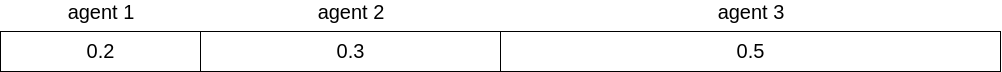
\includegraphics[width=0.75\textwidth,height=0.75\textheight,keepaspectratio]{images/roulette.png}
\caption{This image illustrates roulette selection using three agents and their fitness.}
\label{fig:roulette}
\end{figure}


\subsubsection{Archivists}
Archivists are the modules that write files containing the data of the outcomes into .csv files. They determine what needs to be saved and when that has to happen, while trying to limit resource usage.

\subsubsection{Organisms}
An organism is a container that combines the brain and genomes as well as other components like its ID, time of birth and death and the DataMap which is used to communicate between modules.


\subsubsection{Groups}
Groups are to organisms what organisms are to brains and genomes. They are containers that store the population made up of multiple organisms.

\newpage

\subsubsection{Worlds}
Worlds are the part of MABE that evaluate the organism's performance and contain the fitness function. A world is the environment in which agents compete and it communicates with organisms and their brains and genomes. The world receives the brains outputs, sends back inputs, calling updates and updating states. Just like with brains, worlds are only limited by the power of the system on which they are being run. This applies 1:1 to the physics world as well. Worlds also write into files to track the process. 
Since worlds are generally not limited to many specifics, many different kinds can exist. And so do  fitness functions.

\textbf{What is fitness \& how does it work?} 

Survival of the fittest and natural selection are very well known concepts. Fitness is defined as the mean number of viable offspring, and generally speaking, every behavior or morphological and physiological change that improves this number has a chance to become selected. Imagine an organism that can suddenly hear better due to a mutation. It will now be able to avoid more predators, and thus get more chances to create offspring than other members of its species that do not hear as well. These adaptations in the natural world happen implicitly. Nobody actually counts the mean number of offspring, and thus fitness is simply a natural consequence of mutational effects. In a computational model, we can either implement this implicitly as well (AVIDA uses implicit fitness) or we use what is called an explicit fitness function. The fitness function is used to translate the agent's behavior (we speak of agents instead of organisms in computational models) into a numeral value. Based on this number organisms can now be selected. Fitness can basically be anything we declare it to be. A distance walked by the organism, food found or eaten, offspring created or sheep counted before falling asleep, it can be anything. Then, depending on the fitness function, evolution will take place where organisms with higher fitness have a higher possibility to advance into the next generation.

Fitness can be determined in many ways, if we want to fit a function it would be the root mean square difference we would seek to minimize. In more complex models it would be the performance depending on the task at hand. In foraging it would be the amount of food collected, if the task is to answer questions right, it would be the fraction of correct answers.  

Since there are so many different ways to define fitness, when modeling you have to define fitness yourself which always depends on what you want to achieve with your model and in which way you want your organisms to evolve. The same organism in the same world will evolve differently depending on how you setup fitness.

One of the more common approaches is survival. It is fairly straight forward and self explanatory. If an organism is unable to live, inhabit and survive in the environment that it is given, it and its species will go extinct unless they adapt to the circumstances before they do. This goes back to the Darwinian approach of ``survival of the fittest''.

Sexual Selection is another popular way of implementing implicit fitness. In this scenario, the opposite sexes, mostly the males are trying to appeal to their counterparts and produce offspring in the process. The organisms will evolve in a way to be more and more attractive, whereas the opposite sex will keep on evolving new expectations. Again, a species will most likely die out if it were not for sexual selection, or on the extreme contrary, reproduce without selection and develop unfavorable traits in the process.

We seek to evolve agents in complex environments, where complex means challenging in many different and not necessarily preprogrammed ways. 3D physics would challenge an agent controller to not just abstractly navigate an environment (left right for a pong paddle for example) but it would require the agent to actuate arms and legs for example. However, 3D physics isn't easy which is why we need to use a engine for that.
\textbf{World types}

In a \textbf{Solo World}, the caterpillar world for example, only one organism is being evolved at a time whereas \textbf{Group Worlds} can evaluate multiple agents or even populations concurrently. Using these group worlds even allows for interactions between agents.

Another differentiation which has to be made is between \textbf{Single Generation Worlds} and \textbf{Multi-Generation Worlds}. In single generation worlds, like caterpillar world, after every generation the optimizer is being called to generate the following population. In multi generation worlds this process is being taken care of by the world itself. Some kind of selection process has to be implemented to ``replace'' the optimizer.

\newpage
\section{Complexity}
What most computational tools to study evolution lack, is the ability to evolve virtual organisms that rival natural ones in their complexity. For once, this is due to limited computational resources, but also because designing complex environments to evolve virtual creatures in is difficult in itself. One way out of this dilemma is to use complex 3D physical environments, where the virtual agents now have to deal with the complexity of an actual physical world. 

With such a tool, one would be able to not only study the evolutionary dynamics that other tools allowed but to also address many biological questions that pertain to the morphology and physiology of organisms. The whole field of developmental biology, for example, is concerned with determining how organisms get their physical form. One famous example would be how that happens from a single fertilized egg. Thus, adding this type of capability to MABE~\cite{MABE2016,bohm2017mabe} would expand its capability to facilitate research greatly.

Similarly, many evolutionary hypotheses address the coevolution of brain and body. Just because an organism has claws, does not imply that it knows how to use them to attack or defend itself. The Ankylosaurus (see Figure \ref{fig:Ankylosaurus_dinosaur}) for example had a large bony bulge at the end of its tail (see figure \ref{fig:Ankylosaurus_dinosaur}). Was this a defensive or offensive weapon? And if so, how was it used, or how could this be used? How did it evolve? What are general environmental conditions that lead to such adaptations? These are all questions we would love to answer, but we can not just do that from looking at the fossil. However, in a computer model that contains an evolutionary mechanism and physics, suddenly we can start to answer such questions. While they might not tell us how exactly the past happened, they at least give insights about possible pasts, selection factors, and test the plausibility and likelihoods for certain adaptations to occur. 



\begin{figure}[h!]
\centering
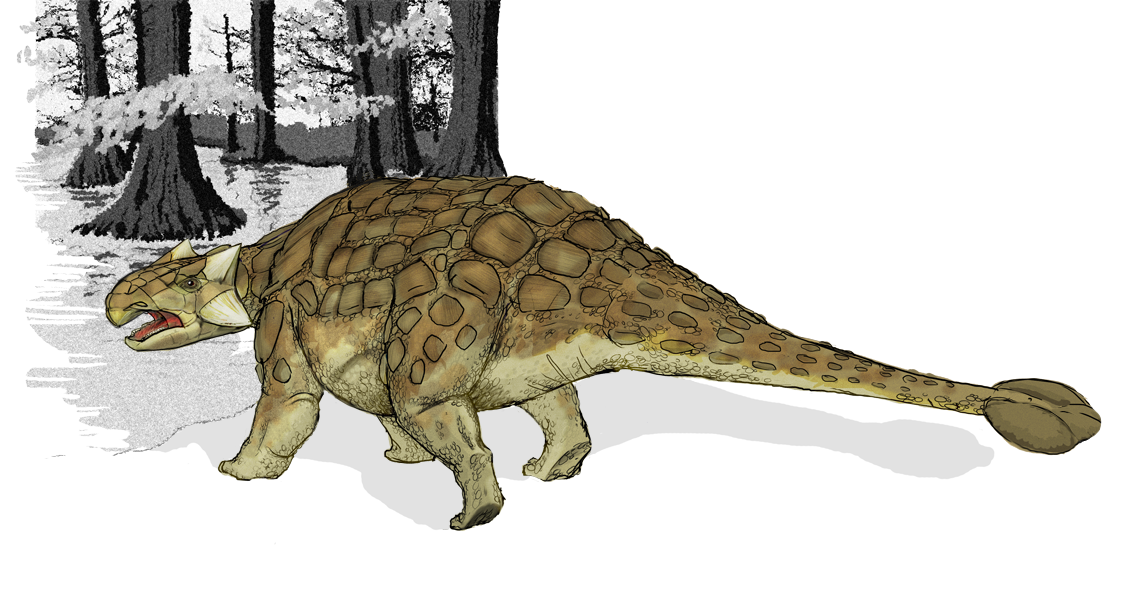
\includegraphics[width=0.7\textwidth,height=0.7\textheight,keepaspectratio]{images/Ankylosaurus_dinosaur.png}
\caption{An image depicting an Ankylosaurus with it's bony bulge on it's tail.~\cite{dino}}
\label{fig:Ankylosaurus_dinosaur}
\end{figure}
%https://en.wikipedia.org/wiki/Ankylosaurus#/media/File:Ankylosaurus_dinosaur.png

\subsubsection{Can we answer questions from the past 100\% accurately that way?}
While making definite answers for what happened in the past might still not always be possible using models, and telling the future also isn't exactly possible, we can make very educated guesses what evolution did and will do and why, given we know the circumstances it all happened under. 

\section{Evolution of Intelligence}

Currently Hintze Lab is interested in general purpose AI, using evolution to achieve that goal. One thing that seems certain is the relation between the complexity of the environment and the degree of intelligence needed to deal with it. Simple environments require simple brains, complex environments need larger brains to deal with them. Since in computational modeling, all environments need to be implemented, creating complexity becomes a cumbersome process. However, 3D physical environments provide a simple platform that allows for complex meaningful interactions to take place, without having to implement them specifically. Simple examples are lines of sights, blending into the background, weight and speed suddenly playing a role, or just the height of an organism providing either an advantage or limiting it's ability. This still has to be coded, but a dedicated physics environment eases the process immensely.

Similarly, Clark~\cite{clark1998being} already proposed the idea that for cognition to evolve, it needs to be \textit{situated}. This means, that the brain not only needs to observe the world, it also needs to act in it. To become an actor, a brain needs a body. Therefore, adding a physics module to MABE is a necessary step towards evolving intelligence.

\newpage

\section{Previous work on embodiment}
Interestingly, the idea to also evolve embodied and not just behavior of brains has been done in the past, for example by Karl Sims who was the first to evolve virtual critters in 3D physics environments in the 80s ~\cite{sims1994evolving}. However, at that time, no specific scientific question was answered, and the work was indeed more of a proof of principle. The goal of this work is to integrate the ability to model 3D physics within MABE and to show how this technology can now be used to carry out experiments regarding the evolution of virtual agents in a complex world. 

\subsection{Karl Sims}
Karl Sims is a computer graphics artist but most famously known for his work and research in evolution of artificial life. In his 1994 film ``Evolved Virtual Creatures'' \cite{sims1994evolving} Sims shows the results he achieved in his virtual evolution research, namely presenting the different critters (see Figure \ref{fig:SimsCritters}) made from simple geometric shapes like boxes and cubes. 
\begin{figure}[h!]
\centering
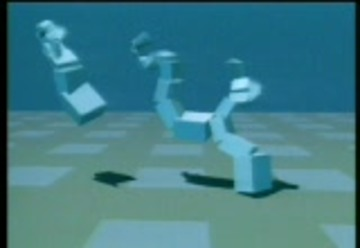
\includegraphics[width=0.75\textwidth,height=0.75\textheight,keepaspectratio]{images/sims_evolved_virtual_creatures_1994&scale=2.jpeg}
\caption{A picture of Sims so called critters, organisms that he virtually evolved.~\cite{critterssims}}
\label{fig:SimsCritters}
\end{figure}
%https://archive.org/services/img/sims_evolved_virtual_creatures_1994&scale=2

Sims counts as one of the forerunners and pioneers in the field of artificial life and its evolution. He has published three papers on the topic in the early to mid nineties. The most critical aspect of his work is probably the evolution of morphology and behavior in a 3D physics environment.

\subsection{Polyworld}
In 1994, the same year in which Karl Sims had released his short film, Larry Yaeger published his initial paper ``Computational Genetics, Physiology, Metabolism, Neural Systems, Learning, Vision, and Behavior or PolyWorld: Life in a New Context'' \cite{yaeger1994computational}, in which he too worked on evolving artificial intelligence. For this he wrote and used his own software called ``Polyworld'' (see Figure \ref{fig:Polyworld}). Polyworld is now open-source and can be found on GitHub, with the latest commit having been pushed in 2016. 
One big advantage that Polyworld has over Karl Sims simulations is that all the code has been published and can therefore be used, studied, analyzed and understood, whereas all of Sims code is written specifically for one machine in Assembly and mostly useless because of that.
\begin{figure}[h!]
\centering
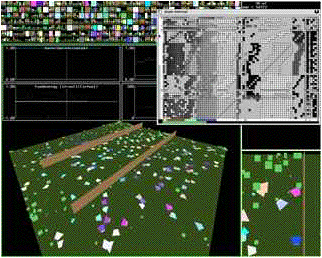
\includegraphics[width=0.75\textwidth,height=0.75\textheight,keepaspectratio]{images/image001.png}
\caption{A screenshot of Polyworld, Larry Yaeger's software to evolve AI.~\cite{polypicture}}
\label{fig:Polyworld}
\end{figure}
%http://shinyverse.org/larryy/Polyworld_files/image001.png

\newpage

\subsection{Framsticks}
Only a couple of years after the release of Polyworld, in late 1996, a new piece of software by the name of ``Framsticks'' (see Figure \ref{fig:Framsticks}) \cite{komosinski1999framsticks} was released by Maciej Komosinski and Szymon Ulatowski. Framsticks is an Ariticial Evolution Simulator too, it is free and features more advanced graphics. It is also being shipped with an optional GUI, which makes it more user friendly, even for people who do not have a background in programming. This makes it more appealing to researchers that originate from the field of biology.

\begin{figure}[h!]
\centering
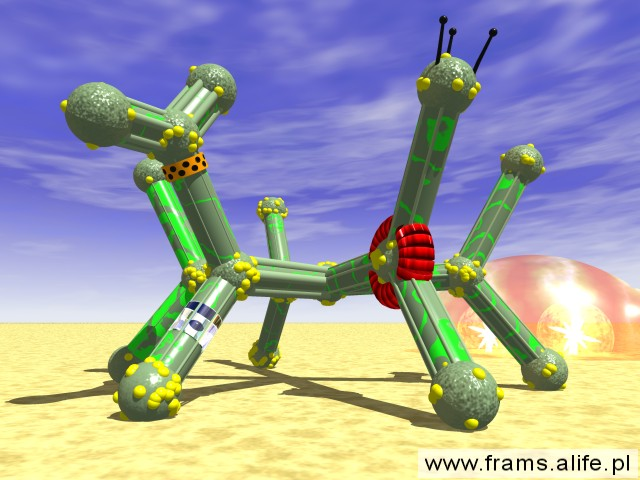
\includegraphics[width=0.75\textwidth,height=0.75\textheight,keepaspectratio]{images/slideD1.jpg}
\caption{A picture of an organism within Framsticks, a tool for artificially evolution.~\cite{frampic}}
\label{fig:Framsticks}
\end{figure}
%http://www.framsticks.com/files/common/slideD1.jpg

\section{Goal: DART integration into MABE}
All of the previously mentioned models are special purpose tools to study one thing. Their results are difficult to share, and they are difficult to change or modify, which is why the Hintze Lab strives to create a tool that runs without all the beforementioned disadvantages. The goal was to create an open source, and therefore free of charge tool. With it being open source and on GitHub for everybody to see, sharing and changing it are as simple as ever. On top of that, MABE is modular and allows for many different blocks to be used. Different Brains and worlds open the door to countless different experiments, which can be fundamentally different.
\newpage
A Physics Engine is a computer program that models real world physics in a nearly perfect fashion in a computer generated and run environment. 
There are many physics engines like unreal~\cite{unrealengine}, unity~\cite{unityengine}, physX~\cite{physxengine}, godot~\cite{linietsky2007godot}, bullet~\cite{coumans2013bullet}, to only count a few, but we use DART~\cite{lee2018dart} because it is free to use, open source, and not very restrictive. DART is also very accurate, which is a trait other engines sacrifice for speed, so that they can be used in entertainment. One thing that many engines do is that they run their own main loop without any exit functions, which means that you can not run your own code to force updates,  pause them or to restart. This would be fairly problematic for what we are trying to do, since the brain and MABE should be in control of the physics steps. The same goes for rendering, most engines just render non stop or not at all. Switching between visualization and text-based is not a very common feature, but dart does come with it, if you opt to use the Open Scene Graph (OSG) rending option. When using OSG, you can control the simulation completely, even from within MABE's world code. 
This shows that DART theoretically has all the features needed MABE to make our experiments run.

\subsection{DART}
DART \cite{lee2018dart} is an open source cross-platform C++ library used for kinematic and dynamic applications for robotics and animation that we are using as our physics engine. It is being developed mainly by the Graphics Lab in collaboration with the Humanoid Robotics Lab, both located at the Georgia Institute of Technology. The Personal Robotics Lab at University of Washington and Open Source Robotics Foundation are also contributing.
DART has been in development since 2011 with version 1.0 being released in 2012. The current release, which we are using as well is version 6.X, which has been free for download since 2016.
Since DART is completely open source, it offers the possibility to look deep inside of whats happening without any restrictions.
DART is available for use and redistribution under the BSD 2-Clause license.

After having looked into DART, having read up on it, having installed it and after testing all the tutorials we agreed that DART is the tool that we want to use and implement into MABE to handle physics as well as visualization. 


\subsubsection{DART's features}

DART in itself provides a huge selection of features that allow for complex and diverse selection of experiments. All the simple features one would expect a physics engine to have, like rigid bodies and collisions are implemented. More complex features, muscles (springs) and joints for examples, are also included and work without any issues. And even soft bodies, which open a wide verity of usage are part of the package that is DART.

\newpage

The following pages will describe how DART was integrated into MABE, including the pre-DART steps, failures, bugs and errors, how one can design environments with it, and how these environments could be used to coevolve the brain and bodies of virtual critters in this 3D physics environment. This is followed by a couple of experiments that first test the integration of Dart into MABE, and then experiments that exemplify how one can use the newly added module to create evolutionary experiments. %This thesis will conclude with findings about how diversity of evolved solutions depends on the complexity of the environment, reaffirming the initial argument that we need more complex environments to study evolution better.

\chapter{Material, Methods, and Implementation}


%\chapter{Implementation}
\section{Godot}
In search for a physics engine, our first stop was Godot \cite{linietsky2007godot}. A free game engine that comes with softbodies in its latest beta releases and  also allows for scripting using C++, which is called gdnative. The first step was to get Godot installed and up and running in both versions, the stable release and the beta, in which we can test with softbodies. The next step was to get somewhat familiar with gdnative, which we did by going through the tutorials and examples given on their official website. 
After all that was done, we had to figure out how softbodies work and how to make them do what we intended. Using the GUI proved most useful during that period in which, after a week of experimenting and testing we finally had to accept the fact that Godot won't actually work, even though it had looked very promising at first. 
The way the testing in godot happened was rather simple. As stated above, we made use of godot's graphical user interface and the ``play'' option, which renders out the scene and applies physics to all the objects. A ``course'' has been set up for the objects to traverse, which means they will fall down a set of slopes (see Figure \ref{fig:Godot}). The goal for this scenario was to create a course that was simple to observe by eye but still complex enough to make it clear if physics are being applied correctly to the soft bodies. There were three slopes, which led to each other downwards, with the objects being spawned above the first slope. This allowed for very simple testing as to how physics operate. %Umschreiben/Ausschmücken

\begin{figure}[h!]
\centering
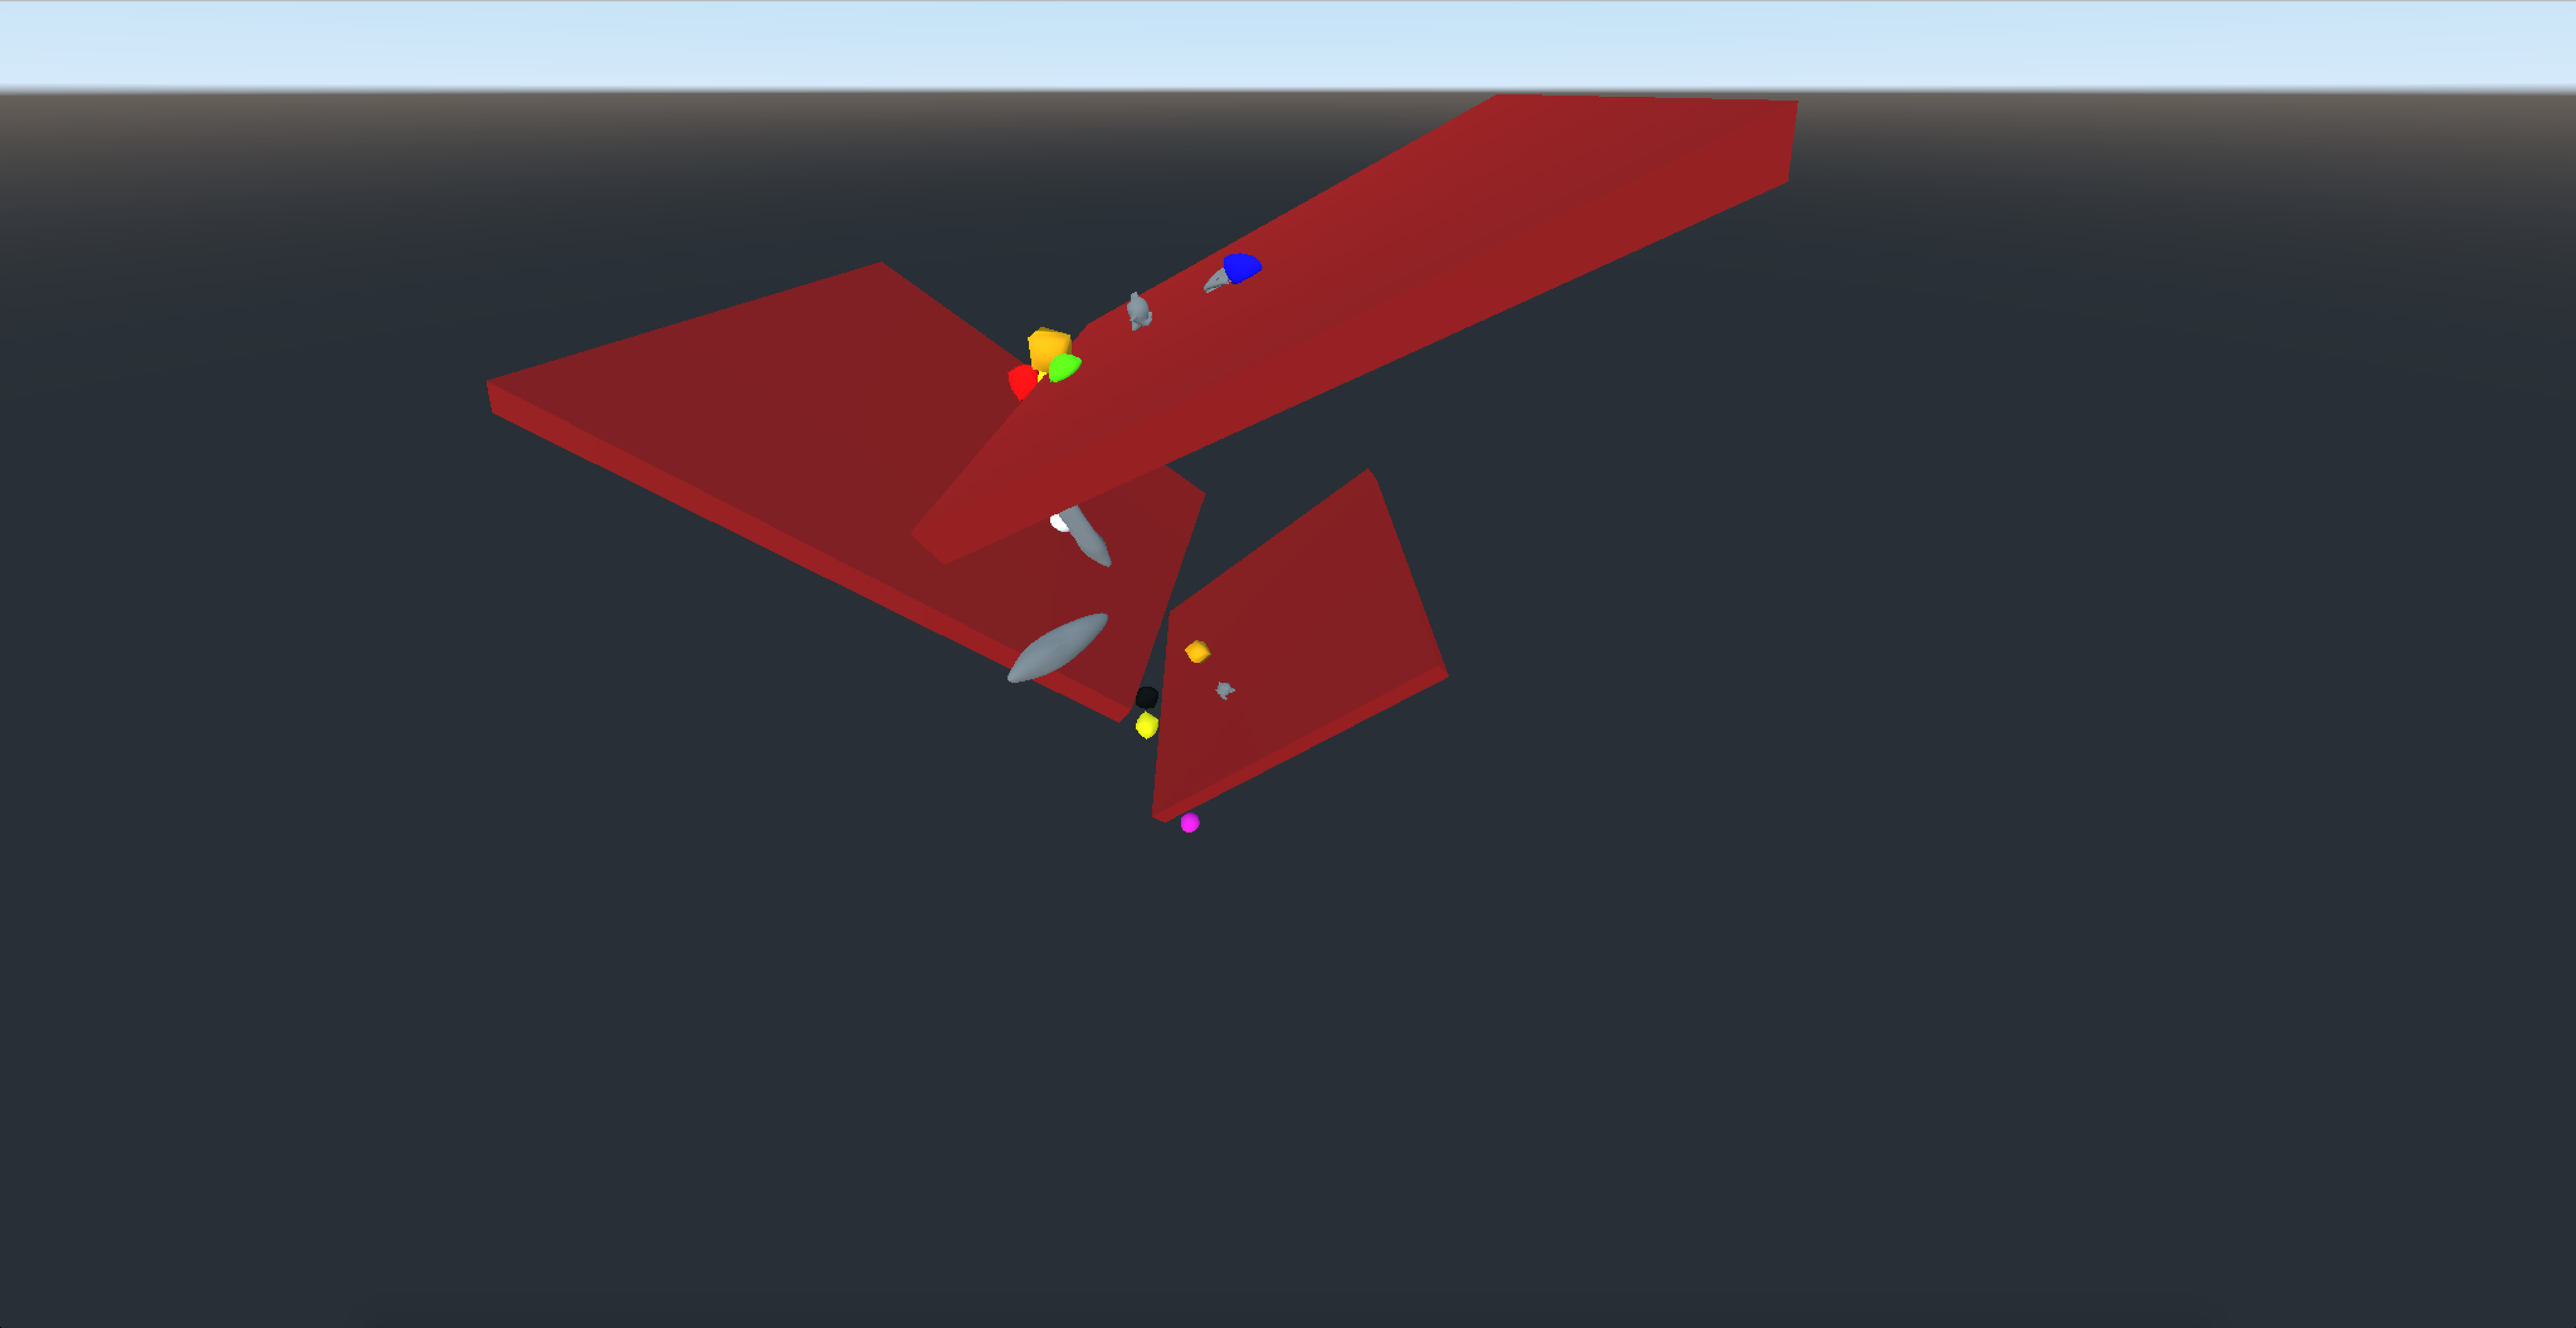
\includegraphics[width=0.65\textwidth,height=0.65\textheight,keepaspectratio]{images/godot.png}
\caption{The godot testing word mid-run. All the objects are falling down the slopes, to be evaluated on their physical behaivior.}
\label{fig:Godot}
\end{figure}

The biggest issue was that while softbodies were able to to interact with rigidbodies physically, they were unable to interact with each other. Also creating a softbody just by itself was not possible within Godot, it always had to come in combination with a ridgidbody inside of it, which defends the purpose of the softbodies in the first place. Another problem would have been modding Godot in a way that would allow us to access the main loop to have MABE control it, which would have meant that we would have had to fork Godot and customize it and recompile it on our own.
%Aufteilen
At this point we agreed that it was not worth the time and effort to continue with Godot.

 After having made the discovery that softbodies have issues we set up a second test ground specifically for the sole purpose of investigating this issue further. This world contained of softbodies with all parameters set in a way for them to be as solid as possible with a very light rigid body falling on them. The rigidbody seemingly ignored the properties of the softbodies and just crushed them without any counter force which proved without a doubt that softbodies were far from sufficient within godot.


\newpage
\section{DART}
\subsection{Pre-MABE testing}
Before implementing DART into MABE, we had to make sure how it works and how it could be implemented into MABE. This process was more difficult than anticipated because DART comes with really poor documentation and outdated tutorials that don't work anymore, on top of a downloadable MAC version that did not install without modifying parts of the code. This in itself took multiple days, just to get anything up and running. Next were the tutorials that I had to also modify and update. After getting them to work I started searching for a simpler and easier project since the work provided by DART was already quite advanced and there was no ``Hello World'' type example available. 
The first small ``project'' we started with was a ball just falling onto a plain. No input, no visualization, nothing fancy. This was really just a project to get a better understanding of what is required and how it works.
Next the phase of implementing glut visualization into this project started (see Figure \ref{fig:ball_example} for the ball example visualized). This was required for the bigger project either way but also let us see if our text-based example really worked, since evaluation physics with text outputs only isn't as easy.


\begin{figure}[h!]
\centering
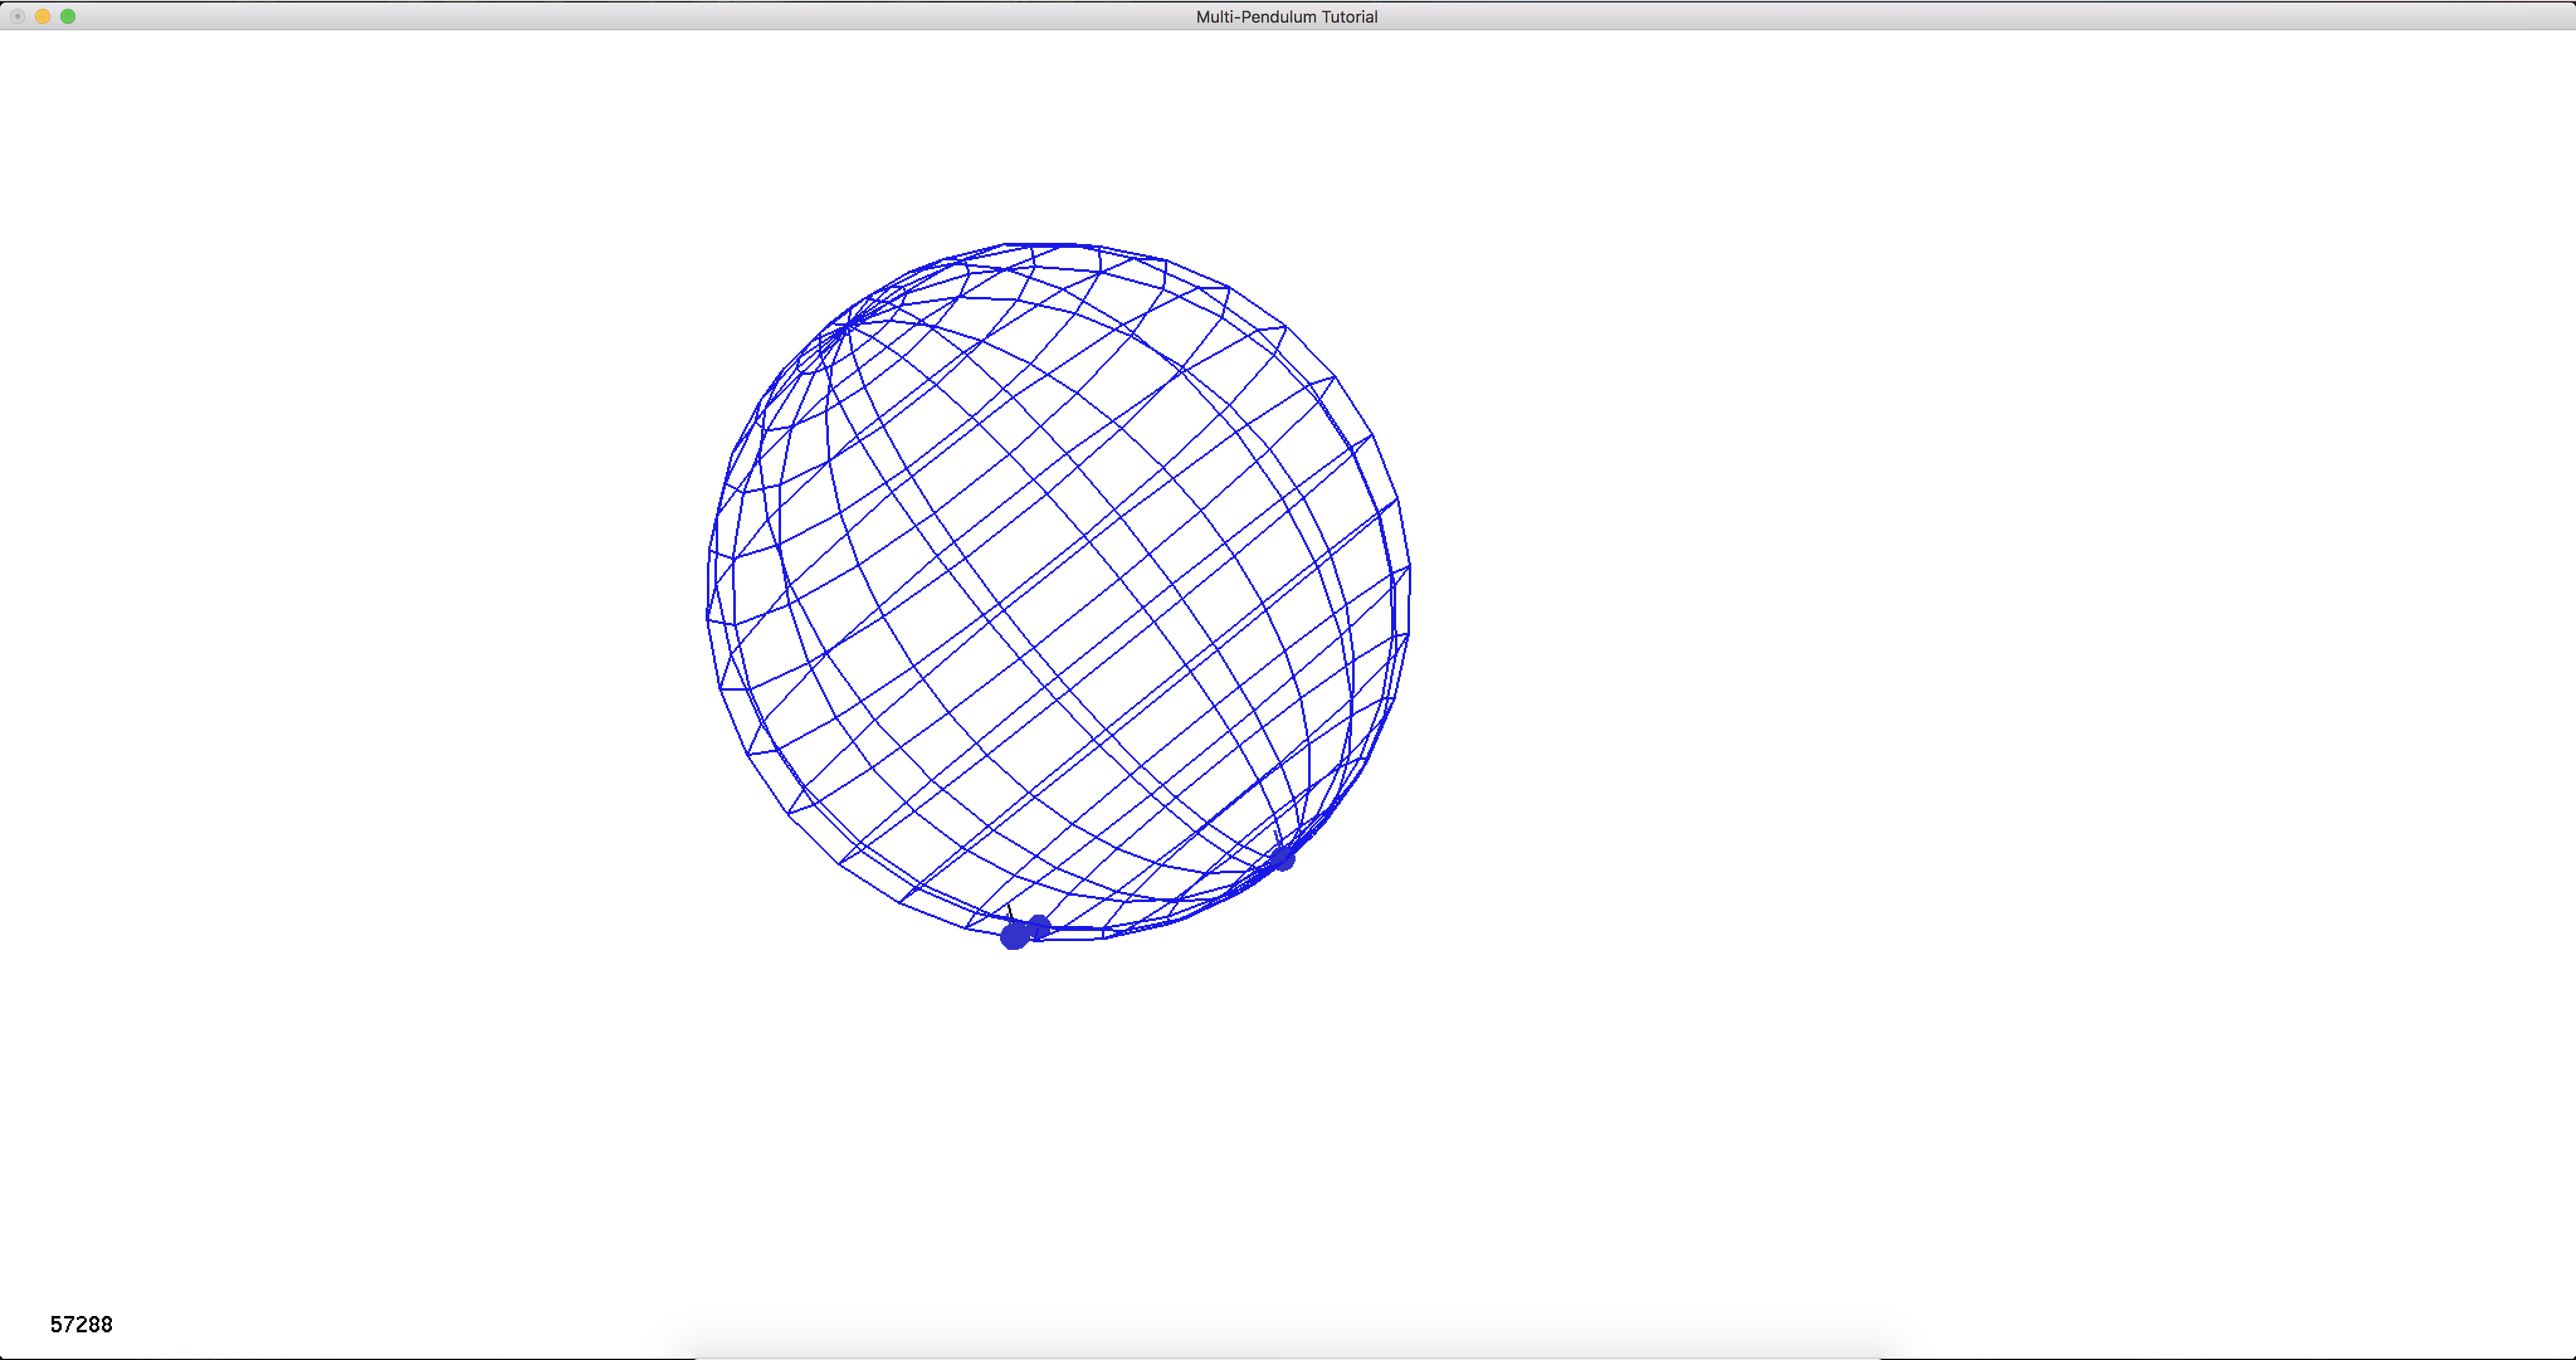
\includegraphics[width=0.65\textwidth,height=0.65\textheight,keepaspectratio]{images/ball_example.png}
\caption{A screenshot of our dart code running the ball testing world with glut visualization turned on.}
\label{fig:ball_example}
\end{figure}

With Visualization now in place, evaluation became a lot easier and now allowed for a visual testing of future components. MABE provides a so called World module which describes the environment in which agents are evaluated.

To create such a module, that integrates DART's methods, and physical elements their properties needed to be established. For example, the ability for agents to push, actuate muscles, inputs from sensors, or how the entire environment could be reset. 
Additionally, how fitness functions could be defined within DART had to be explored for an agent-based program such as MABE. For that, a debug feature was implemented. This feature allows users to take the role of the brain and control the agent through keyboard button presses. This allows future users to try out DARTs interactive capabilities, and simplified further integration.

Again, due to poor documentation, finding the right functions for the things we were looking for was rather difficult and this was true throughout the entire project. For example, to push the ball, multiple things need to be set, known, and controlled: the order of the coordinates in the set and force functions, which is (yaw, pitch, roll, x, y, z) and to get a feel for which forces are required or suitable for this easy task, as well as just figuring out which function actually executes code that does what we think and want it to do. 

We found this to be a good way to just see how physics behaved and how realistic they felt to the human eye in order to see if there were any obvious discrepancies, which there were none to speak of.

\subsection{Integration into MABE}
Firstly and mainly, implementing DART into MABE meant reducing the DART example code to the bare minimum, without getting rid of any of the necessities. 
In this case, visualization would not be enabled or used at first. This simplified things a lot, which would help during the process of merging the two projects into one whole. The code we used was the ``ball falling onto a plain'' code, which would later become the ``Ball Pushing'' World. But so far it was just the simplest, most bare bone piece of code available to us. 
Determining what was needed was a lot easier with this rather small program, and thus the merging process started. Figuring out which part of the MABE World module should hold which part of the DART code was the first challenge, with linking being the far more time consuming step that followed right after. 

\subsubsection{Bugs}
The first problem encountered was rendering. By default DART used glut for visualization. Using this option allowed for visualization to work just fine, but exiting out of the main visualization loop was impossible. Once entering that loop there was no exiting it after, which meant that there was no way to run more than one organism, which defeats the purpose of genetic programming completely. Trying to use freeglut instead proved to be another unsuccessful approach. Instead, we went with another rendering option that DART ships with: OSG. This meant re-linking the whole project again and switching out the code for visualization, but after all that was completed, we were able to step everything on our own accord.

Variation of the time defining a physics step affected the results greatly. Consequently the default values were used thereafter. It still was possible to modify it using the config files. This should be done with caution, especially within a series of experiments since it could heavily affect the outcome. 

Heavy memory leakage was encountered at first after we had implemented visualization, since a new window was spawned for every single agent. This allocated new memory incredibly fast. The way of solving this was to not spawn new windows, but to instead reuse the same window for each organism and generation. Also, instead of creating new worlds we reset the current world and the organism in it. This way no new memory is being allocated and no memory leak was being created. 


We had encountered a bug after getting visualization to work in which the results of the visualized version varied heavily from the text-based results, even though all the parameters and settings were the same. The results should have been 100\% identical, but they were not. This would obviously render the whole idea of being able to switch between visualization and text-based obsolete and it meant that one of the two options was flawed immensely. First we had to find out which of the two options was broken. To do that, falling back to the manual test code examples and testing both versions with the same code was necessary. It turned out that the text-based option was the one that wasn't working correctly. Then we had to figure out why exactly that was. As it turned out we just had to comment out a single function call that was still in place from one of our example projects that was stepping the engine further in a place where it should not have been.
After removing that line from the code and rerunning a few tests the problem was fixed and both versions were then giving us the same results.


\section{A DART World}
To run successful experiments in MABE using DART we need many different components. Beyond implementing inheritance (Genomes), variation (Genomes, and Optimizers) and selection (Worlds, Brains) MABE provides additional components to support research: line of decent tracking (Archivist), setting parameters (Parameter system), running multiple jobs (MQ), a built system (MBuild), and generational tracking (Populations/Groups). What DART needs to provide for our experiments to function is the world itself including the physics environment. MABE can then use this world to determine the fitness (performance) of each agent. With this evaluation, all other components can now proceed to evolve the popultion of agents. A world in the MABE sense, which means an environment in which evolution can happen, and a physics world, are not synonymous, since a MABE world also controls fitness, handles the brain in- and outputs and more. So the ``world'' in DART is only part of the world that MABE accesses.
But that we still have to set up. 
We don't really need to set up the world itself, using only one command (\textit{world = dart::simulation::World::create();}) is sufficient already. In DART we always start off with an empty ``world'', but what we do need to do is fill the world with the elements we need for our experiments.


\subsection{How to set up an object in DART}
In DART, every object consists of the same basic ``blocks''. For each object, even if you just want to create a plain and simple cube or sphere (see Listing \ref{lst:creatingsphere}), you will have to start of with a skeleton. A skeleton in dart exists to potentially connect and group of multiple objects and joints into a bigger whole. But even if only one object is being spawned, a skeleton is required, it will only hold a single BodyNode in this case, but it is still needed. 
A BodyNode consists of two main components, the BodyNode properties and the joint properties. These are being combined into a pair, which then holds the objects shape, mass, collision, color and all the other aspects defining the object itself. Again, just like with the skeleton, every object needs a joint, even if the object is not connected to anything. In that case a FreeJoint will be used, which gives the object 6 degrees of freedom and it will behave like a ``free'' physics object within the world. 
Of course BodyNodes can also be attached to other BodyNodes using joints. 
\begin{lstlisting}[language=C++, label={lst:creatingsphere}, caption=Creating sphere in DART]
int radius = 2;
dart::dynamics::SkeletonPtr sphere = dart::dynamics::Skeleton::create();
sphere->setName(``sphere'');
dart::dynamics::FreeJoint::Properties sphere_joint_prop; 
dart::dynamics::BodyNode::Properties sphere_body_prop; 

std::pair<dart::dynamics::FreeJoint*, dart::dynamics::BodyNode*> sphere_pair =
sphere->createJointAndBodyNodePair<dart::dynamics::FreeJoint>(nullptr, sphere_joint_prop, sphere_body_prop);

dart::dynamics::ShapePtr sphere_shape(new dart::dynamics::SphereShape(radius));

auto shapeNode =
sphere_pair.second->createShapeNodeWith<
dart::dynamics::VisualAspect, 
dart::dynamics::CollisionAspect,
dart::dynamics::DynamicsAspect>(sphere_shape);

shapeNode->getVisualAspect()->setColor(dart::Color::Blue());

Eigen::Vector6d positions(Eigen::Vector6d::Zero());
sphere_pair.first->setPositions(positions);

world = dart::simulation::World::create();
world->addSkeleton(sphere);
\end{lstlisting}

This code example creates a sphere that is connected to the world by a FreeJoint and is therefore free to move anywhere.
\lstinline{sphere->setName(``sphere'')} might seem unimportant, but it is not. Names have to be unique, or they will later automatically changed by DART when adding the skeleton to the world. The same thing happens when adding BodyNodes to the skeleton. Unique names are required and will be set automatically when they are not being defined by the user, but this generates warning messages during run time, which is not ideal of course. So setting them is something that should not be forgotten.
As explained above, we will make use of the FreeJoint for this sphere, since we want it to fall freely, unattached to anything in the world.
When declaring the shapeNode you can see that it holds control over whether it should collide with other objects (\lstinline{dart::dynamics::CollisionAspect}). Leaving \lstinline{dart::dynamics::CollisionAspect} out will make the object no-clip with other objects, meaning it would not collide or interact physically with anything in the world and behave as if would be alone. In this case this is not desired, so \lstinline{dart::dynamics::CollisionAspect} will be included in our shapeNode setup.

%JUMPHERE

\subsection{Results}
The test was a success. Inputs worked without any issues, as did the experiment itself. The ball fell to the ground right after being spawned/reset and could then be pushed in all directions, except up and down, which is exactly how it should be. Since this code was still run in its own, without MABE being involved with it at all, it is a great proof of concept to show that DART can handle ``evolvable'' worlds and environments.  This will allow for a good test setup within MABE, once integrated.  

After having run the test in DART on its own it was time to test it in combination with MABE. Pushing buttons by hand to make things happen, like moving the ball in the ball pushing world was no longer our goal and no longer acceptable. We now had to get MABE to do that for us.


\newpage

\section{Experiments}
\subsection{Ball Pushing}
After understanding how DART works and how we could set it up in the way we'd like, we had to somehow implement it into MABE so that the two could work as one, so that MABE could take control over DART and let evolution do it's thing in the physics environment. We no longer wanted to push buttons ourselves, we wanted MABE to do that for us and for it to optimize that using evolution. First we would have to set up a way to define fitness. In this world, which we will call BallPushing, fitness is fairly straight forward. It is the distance the ball is being pushed into the positive direction on the x-axis. No restrictions or special exceptions, no fancy formulas, just the distance. We gave MABE control over the pushing mechanism. It had the power to push the ball on two degrees of freedom, those being the x and y axis. You can think of it as if MABE is using its ``finger'' to push the ball with a force parallel to the ground in any direction with a variable force. The brain was giving us two outputs every so many frames, we had set up a parameter for how many that should be, as well as simulation speed and length which could be set in the settings too. We let MABE run with a population size of 100 through 1.000 generations and it proved to be successful. MABE was able to run through all the physics instances without any complications, which successfully showed us that our plans were possible. This short and easy example is a working proof of concept in a very simple environment, which was the first stepping stone for the next experiment: a more complex environment in which MABE will be tested on a more complex problem.

\newpage

\subsubsection{Ball Pushing results}
After having gone through all 1.000 generations MABE was seemingly maxing out the fitness. And only mutations would vary from it. All this happened in very few generations, which could be explained by the lack of complexity this world had to offer.


\begin{figure}[h!]
\centering
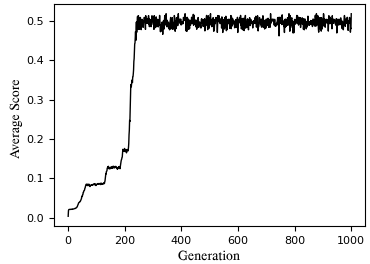
\includegraphics[width=0.75\textwidth,height=0.75\textheight,keepaspectratio]{images/ballgraph.png}
\caption{The results of the Ball Pushing world after having it run for 1.000 generations.}
\label{fig:ballgraph}
\end{figure}

\subsubsection{Ball Pushing conclusion}
Since this world is so easy and straight forward, and since MABE only had to generate two outputs, MABE soon figured out the ideal way of pushing the ball, which obviously was using the maximum force in direction of the positive x-axis. Once it reached that point, it maxed out and just stayed in that area.

\newpage

\subsection{Caterpillar}
\subsubsection{The static virtual Caterpillar}
When we say caterpillar we are of course not talking about a 100\% accurate representation of the juvenile stage of a butterfly. The construct within MABE, however, remotely resembled one (see Figure \ref{fig:Caterpillar}). The caterpillar consisted of five individual body parts. Body parts were cuboids of which each of them was connected to the other two adjacent parts around it with a joint that was controllable by the brain, or rather the ``muscles'' were. The caterpillar as a whole was a physics object connected to the world with a free joint and therefore completely unattached to anything. That meant, while all the body parts were sticking together, the caterpillar was not connected to any world object or any other objects outside from itself. The caterpillar's goal was very similar to the goal we had set in the ball pushing world before, distance in the x direction equals the fitness. The only difference this time was that we had to calculate the average of all the body parts positions, since the caterpillar was a more complex object than the ball. Therefore the caterpillar would evolve a way to ``walk'' and gain distance. In the first set up it had ten seconds of time to move, a population size of 100, and 250 generations to evolve.
\begin{figure}[h!]
\centering
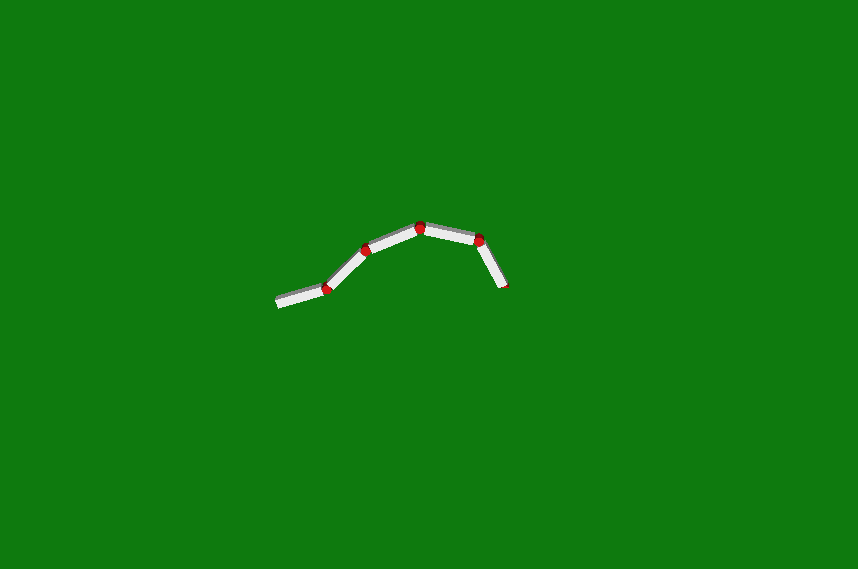
\includegraphics[width=0.75\textwidth,height=0.75\textheight,keepaspectratio]{images/caterpillar.png}
\caption{A picture of a moving caterpillar during the experiment.}
\label{fig:Caterpillar}
\end{figure}

\newpage

\subsection{The caterpillar's ``muscles''}
We were using ``RevoluteJoints'' for the caterpillar body part connectors, these allowed for 1 degree of freedom, that being rotation in the given direction, in our case up and down. But joints alone would not do the trick, since they only allowed for movement to happen, but without setting them up right and giving them the right values and setting the right parameters, they would not move on their own. 
To accomplish actual movement from within the body itself, not from the outside like we did with the ball, we had to make use of the joints spring capabilities.
First, we'll detail how we went through each joint and then through each of their DOFs to set the position limits (see Listing \ref{lst:settinglimits}) and the spring stiffness. The limits are being set in radians and limit the joints movements in either direction after the given point has been reached. 
Spring stiffness sets the springs force. The higher the value the stronger is the spring.

\begin{lstlisting}[language=C++, label={lst:settinglimits}, caption=Setting Limits]
  for(std::size_t i = 1; i < pendulum->getNumJoints(); ++i)
  {
    pendulum->getJoint(i)->setPositionLimitEnforced(true);
    for(std::size_t j = 0; j < pendulum->getJoint(i)->getNumDofs(); ++j)
    {
      pendulum->getJoint(i)->setSpringStiffness(j, 255);
      pendulum->getJoint(i)->setPositionLowerLimit(j,-1.5);
      pendulum->getJoint(i)->setPositionUpperLimit(j,1.5);
    }
  }
\end{lstlisting}

Once these values were set we could ``safely'' control the caterpillars ``muscles''. To do that we set values for the rest position (see Listing \ref{lst:settingforce}) variable of the joints DOFs. Again we looped through all the skeletons joints and then through all their DOFs. But this time we set the rest position. This emulates muscles for us, as it will change the springs length dynamically and therefore contracts or expands our ``arms'' or body parts of the caterpillar. Values could be either positive or negative, the higher the more power was being applied in the positive direction and vice versa.

\begin{lstlisting}[language=C++, label={lst:settingforce}, caption=Setting Force]

  for(int i = 1; i < skel->getNumJoints(); i++)
  {
    for(std::size_t j = 0; j < skel->getJoint(i)->getNumDofs(); ++j)
    {
      skel->getJoint(i)->getDof(j)->setRestPosition(outputs.at(i-1));
    }
  }
\end{lstlisting}

\subsection{The caterpillar's brain}
Muscles and a body already made the rendering look the way we wanted it to, like a  caterpillar, but it did not yet move or function like one, or like whatever MABE, the brain, and evolution think was best. 

The brain is what actuates and controls everything and what pulls the strings.
The way it was set up in this world, the brain did not have the power to control the caterpillar at any time, at any physics update. Instead we had set a parameter that could be set in the settings\_world.cfg that controls how often per second the brain had the ability to influence the caterpillars muscles. 
Each joint received its own output from the brain, which was then being applied to the setRestPosition function for the chosen joint. 

The brain also received inputs every time the brain output values. The input was the sin of time, which let the brain know when it used which output and let it relate the value to the time.

After having given the brain the input, the caterpillar's movement became a lot more coordinated. Before the movement was very choppy and random, and only after the inputs were being handed to the brain did it seem to be able to make sense of what was going on. 

The movement resembles the movement of a 1mm long C. elegans nematode (see Table \ref{tab:elegans}) as in how it also uses a wavy motion to go forward.

{\centering
\begin{table}[ht]
\begin{tabular}{cc}
\begin{subfigure}{0.4\textwidth}\centering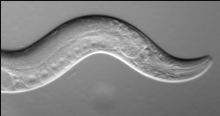
\includegraphics[width=0.75\columnwidth]{images/Caenorhabditiselegans0A1.png}\caption{First Frame}\label{fig:eleganstaba}\end{subfigure}&
\begin{subfigure}{0.4\textwidth}\centering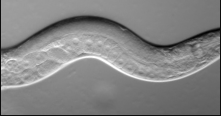
\includegraphics[width=0.75\columnwidth]{images/Caenorhabditiselegans0A2.png}\caption{Second Frame}\label{fig:eleganstabb}\end{subfigure}\\
\newline
\begin{subfigure}{0.4\textwidth}\centering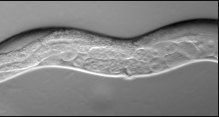
\includegraphics[width=0.75\columnwidth]{images/Caenorhabditiselegans0A3.png}\caption{Third Frame}\label{fig:eleganstabc}\end{subfigure}&
\begin{subfigure}{0.4\textwidth}\centering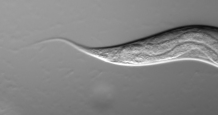
\includegraphics[width=0.75\columnwidth]{images/Caenorhabditiselegans0A4.png}\caption{Fourth Frame}\label{fig:eleganstabd}\end{subfigure}
\end{tabular}
\caption{A 1mm long C. elegans nematode's movement displayed step by step in four still images.~\cite{crawling}}
\label{tab:elegans}
\end{table}
}
%https://en.wikipedia.org/wiki/Caenorhabditis_elegans

\newpage

\subsubsection{Resseting the brain and world}
Since each time an agent ``dies'', which happened every 4 seconds in my experiments, the world should just reset. But there is not just a one stop function that solves this problem, and spawning in a new world each time is just incredibly poorly performing. To get around the issue we used a number of functions (see Listing \ref{lst:resetting}). Each reset parts that then combined to give us the result we wanted. \lstinline{brain->resetBrain()}, just like the name suggests reset the brain, \lstinline{physicsWorld->step(true)} stepped the physics ahead once, but the true parameter tells it to reset the world while doing it. This alone was not sufficient, but in addition with the following functions it worked. \lstinline{physicsWorld->reset()} reset the world's internal counter and time back to zero. With the for loop we accessed the Objects location and set it back to zero where it started, so that there is not continuous progress due to spawn locations. \newline \lstinline{physicsObject->getDof(5)->setPosition(starting_height)} resets the agent back to its starting height, since each time it spawned from a bit up in the air. This overwrote the Z position of the function called before.
\lstinline{physicsObject->resetVelocities()} and \lstinline{physicsObject->resetAccelerations()} were pretty much self explanatory and did just what their name implies.
\begin{lstlisting}[language=C++, label={lst:resetting}, caption=Resetting world and brain]
    brain->resetBrain();
    physicsWorld->step(true);
    physicsWorld->reset(); 
    for(int i=0;i < physicsObject->getNumDofs(); i++)
    {
      physicsObject->getDof(i)->setPosition(0);
    }
    if(numberOfOutputsPL->get(PT)%2 != 0)
      physicsObject->getDof(3)->setPosition(-((numberOfOutputsPL->get(PT)/2)*((jointLengthPL->get(PT)+default_width))));
    else
      physicsObject->getDof(3)->setPosition(-((numberOfOutputsPL->get(PT)/2)*((jointLengthPL->get(PT)+default_width)))+((jointLengthPL->get(PT)+default_width)*0.5));
    physicsObject->getDof(1)->setPosition(M_PI/2);
    physicsObject->getDof(5)->setPosition(starting_height);
    physicsObject->resetVelocities();
    physicsObject->resetAccelerations();
\end{lstlisting}

\newpage

\subsection{Code}

After making the decision that the amount of body parts should be equal to the number of outputs from the brain we had to change the way body parts were being added to the skeleton as well as how forces were being applied to each joint. Before it was all coded static and run through loops with fixed numbers, which worked temporarily but had no right being in the final project. The outputs were all each assigned to their own variable which too was just a quick and dirty way of passing them forward, but was insufficient once you wanted to change the number of body parts. 
\begin{lstlisting}[language=C++, label={lst:setup}, caption=Dynamic Caterpillar setup]

for(std::size_t i = 1; i < pendulum->getNumJoints(); ++i)
  pendulum = Skeleton::create(``pendulum'');
  pbn = makeRootBody(pendulum, ``body1'');
  std::string bodyname = ``body'';
  for(int i=0; i<numberOfOutputsPL->get(PT); i++)
  {
    bodyname = bodyname + std::to_string(i+2);
    pbn = addBody(pendulum, pbn, bodyname);
  }
\end{lstlisting}

The pendulum, which was the name of the skeleton, as well as the ``RootBody'', were being called before the loop and just once. The RootBody counts as the first bodynode but basically just connects the skeleton to the world. After that we added the amount of bodynodes we would like to it by calling the addBody function (see Listing \ref{lst:setup}). Bodyname is just a standard string so that all the bodynodes hold distinctive names.

\newpage

\begin{lstlisting}[language=C++, label={lst:outputs}, caption=Dynamic Brain Outputs]
 for(int i=0; i<numberOfOutputsPL->get(PT); i++)
        {
          brainOutputs.push_back(brain->readOutput(i));
        }
        applyForce(physicsObject, brainOutputs);
\end{lstlisting}

\lstinline{brainOutputs} is a standard template library vector and will always hold as many \lstinline{double} values as the brain gives outputs and then pass on the vector to the applyForce function along with the object which should be affected, in our case this is the caterpillar (see Listing \ref{lst:outputs}).

\begin{lstlisting}[language=C++, label={lst:force}, caption=Force application]
void PhysicsWorld::applyForce(dart::dynamics::SkeletonPtr skel, std::vector<double> outputs)
{
  
  for(int i=0; i<outputs.size(); i++)
  {
    if(outputs.at(i) > 1.5)
      outputs.at(i) = 1.5;
    else if(outputs.at(i) < - 1.5)
      outputs.at(i) = -1.5;
  }
  
  for(int i = 1; i < skel->getNumJoints(); i++)
  {
    for(std::size_t j = 0; j < skel->getJoint(i)->getNumDofs(); ++j)
    {
      skel->getJoint(i)->getDof(j)->setRestPosition(outputs.at(i-1));
    }
  }
}
\end{lstlisting}
One thing that isn't ideal is the first for loop here, where we check the outputs vector to not be higher or lower than a certain value. Technically this is what the functions ``setPositionLowerLimit'' and ``setPositionUpperLimit'' are for. And they do work, but every time a value over the set limits is being applied, instead of just setting it to the limit, it also prints out warning messages, which overwhelms the console. Therefore, I started to also adjust the values by hand (see Listing \ref{lst:force}).

\newpage

\subsubsection{Fitness function}
The fitness function for the caterpillar (see Listing \ref{lst:fitness}) is not very long or complicated. Agents were being scored on the traveled distance on the x-axis.

%Sollte easy sein, aber evolution cheated, daher jetzt so:
\begin{lstlisting}[language=C++, label={lst:fitness}, caption=Fitness Function]
double mean = 0;
    for(int i=1; i<physicsObject->getNumBodyNodes(); i++){
      mean += physicsObject->getBodyNode(i)->getWorldTransform().translation()[0];
    }
    mean = mean/physicsObject->getNumBodyNodes();
    double score = -mean;
    if (score < 0.0)
      score =  0.0;
    if (isnan(score))
      score = 0.0;
    double height = 0;
    for(int i=1; i<physicsObject->getNumBodyNodes(); i++){
    physicsObject->getJoint(i)->getPositions() << std::endl;
      height += physicsObject->getBodyNode(i)->getWorldTransform().translation()[2];
    }
    height = height/physicsObject->getNumBodyNodes();
    if(height > 3)
      score = 0.0;
    org->dataMap.append(``score'', score);
\end{lstlisting}
First the mean of all the joints is being calculated, in an effort to prevent the caterpillar from just stretching one joint out as far as possible to get a quick score on which it then stabilizes. 

The reason for the mean being set to its negative is because the caterpillar's head was being spawned in facing towards the negative of the x-axis and we preferred it to walk forward, so we decided to just flip the score over. 

The reason for why there is a isnan check is because MABE, or GA's in general, over time always find a way to exploit code. This also happened here when we ran it the first few times. It always found a way to catapult its way out of bounds into NAN territory where it would then stay for all the following generations. Even though this result was technically the perfect score, it was not really what I wanted and it did not really allow for any more experimenting, so I made it that NAN equals no score.
\newpage
Also, if the caterpillar moved backwards, which would theoretically then result in a negative score, the score would be set to 0. This is due to the fact that MABE can not handle negative scores. Also, going backwards should be discouraged no matter what, so setting it to 0 right away still makes sense, while simplifying things for the coder and the end user.

The last exception which was encoded was that we set a limit for distance above the ground. This goes hand in hand with the NAN check just before. The way the caterpillar reaches NAN was by leaping high and far through the air, therefore reaching a high distance in both directions. By limiting the vertical distance at the point of scoring, it can no longer just ``fly off'', which also is a decision we made to be able to evaluate the process of movement evolution.
\subsection{Caterpillar results}

\begin{figure}[h!]
\centering
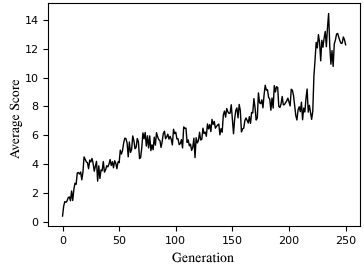
\includegraphics[width=0.75\textwidth,height=0.75\textheight,keepaspectratio]{images/Score_Caterpillar.png}
\caption{The graph displaying the caterpillar's score over time throughout all generations.}
\label{fig:scorecaterpillar}
\end{figure}

As we can see (see Figure \ref{fig:scorecaterpillar}), the caterpillar progressively increases its score over time, after averaging close to nothing to begin with. As time progresses we can see that the score reaches its peak at around the 225th generation. 
\newpage
\subsection{Caterpillar conclusion}
We ran the caterpillar evolution for 250 generations with a population size of 100. Just like expected, at first, the movement and coordination were abysmal and the caterpillar was just flopping around, but as the second generation kicked in, improvement was immediately  noticeable. 

One thing that might seem a bit strange at first was, when seeing the final generations, that while it did somewhat resemble a caterpillar in it's basics, it was far from what you might expect it to be. It moved mostly in the wavy manner, like a 1mm long C. elegans nematode, or even somewhat similar to real caterpillars, but it ``abused'' DART and the physics environment as much as it was allowed to do so.

There are certain restrictions setup for it not to go and cheat the engine, but it still finds a way. Since the modelled caterpillar is not 100\% accurate, or even close, it isn't really meant to be anyways, the model couldn't even move like a real caterpillar would. But what MABE soon figured out was, that the caterpillar was fairly strong, once a certain amount of upwards momentum was created, it then used that to catapult itself for a reasonable distance, which made up a fairly big portion of its score.

\subsection {Manual Morphology - Finding the perfect Parameters}
We have shown that the implementation works and that it successfully evolved our caterpillar like organism to a state where it could easily move. The whole system was even capable of fairly easily changing the caterpillars amount of body parts, and the length of those body parts. These two dynamic changes mentioned are not yet working in run time though, which is why we will compare them ``by hand'' for now. We will use a MABE script that lets us run the ``same'' experiment with different parameters and seeds in a row, so as to compare them after. We ran a population size of 100 for 250 generations with 50 iterations for each to generalize the result for each of our setups. The world stayed the same, and so did the fitness function. Score would still be obtained by walking on the x axis. And the organisms were being scored on mean of all the joints, so being longer was not necessarily an advantage just because the tip spawns further out.

\newpage

\subsection{Number of Body Parts}
We will begin with the number of elements our caterpillar was made out of. We let MABE run through the options of two, three, four, five, six, and seven (see Figure \ref{fig:parts_bars}). Except for the seed, none of the other variables changed. We strongly expected the number of parts to have a strong impact on the caterpillar's performance, but it was hard to guess which option out of the six given would actually prevail. 

\begin{figure}[h!]
\centering
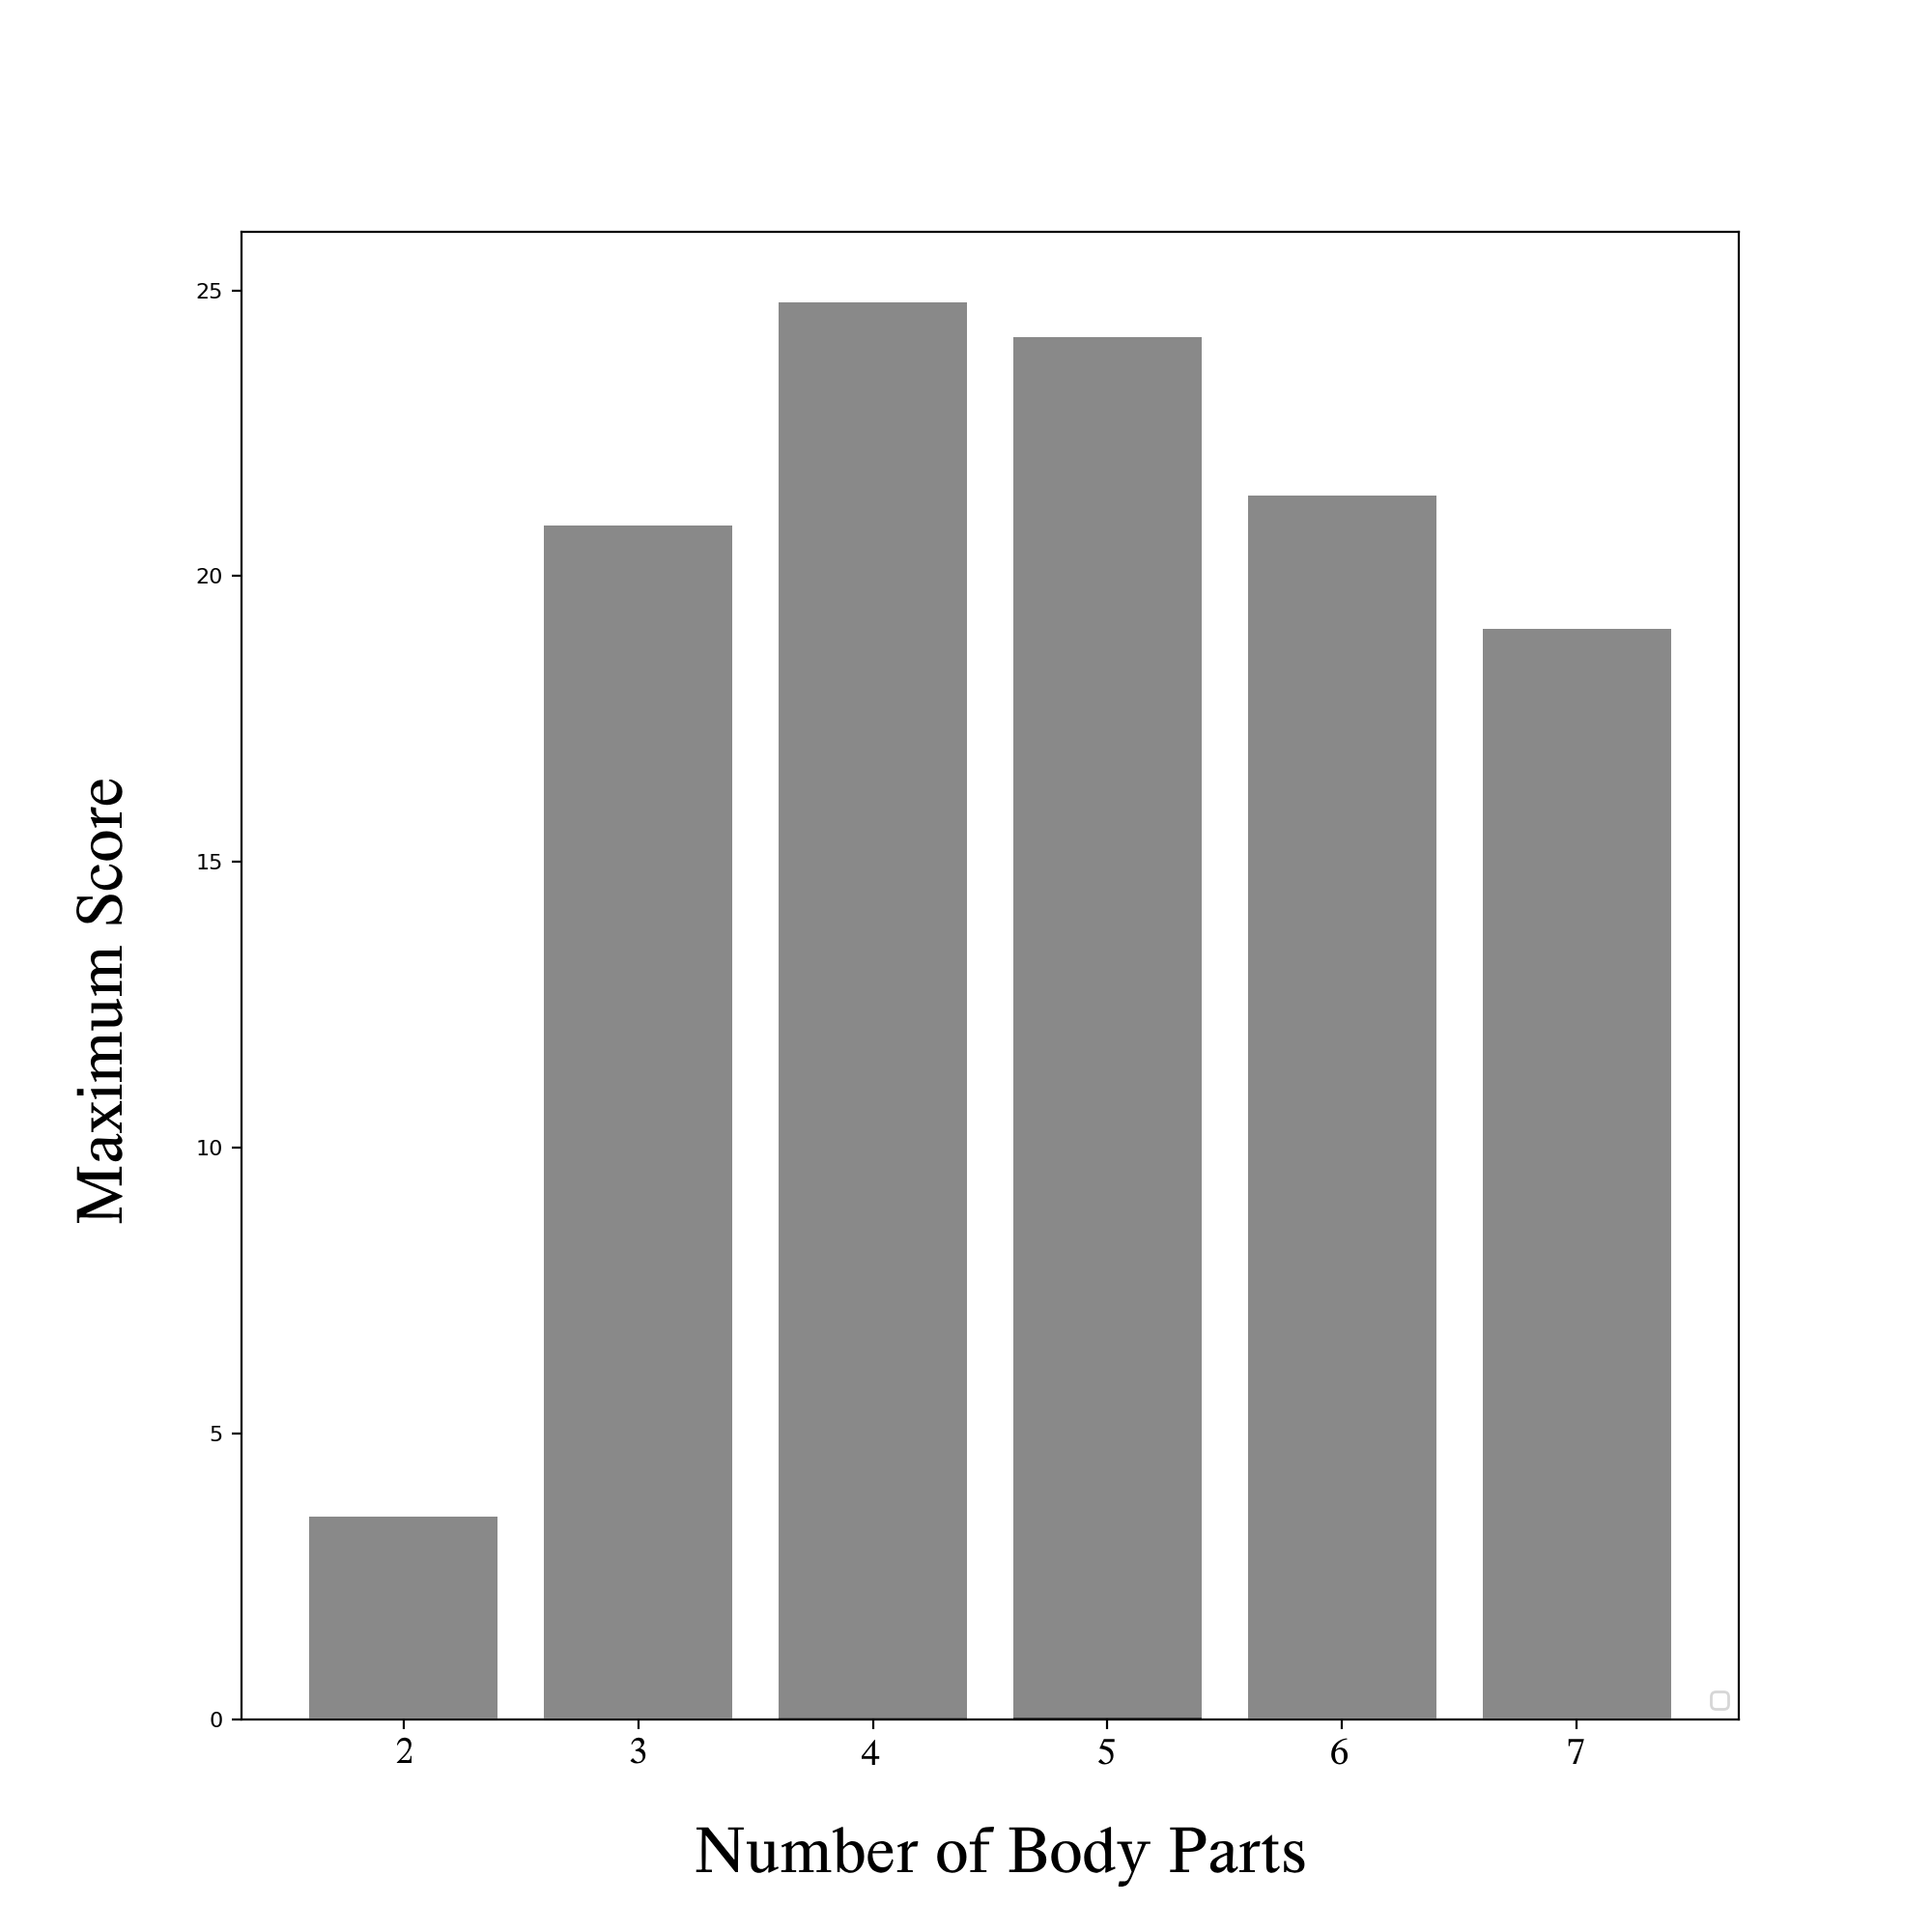
\includegraphics[width=0.75\textwidth,height=0.75\textheight,keepaspectratio]{images/parts-bars.png}
\caption{Bar Plot displaying average score for each amount of bodyparts that was tested}
\label{fig:parts_bars}
\end{figure}

%IS THIS RIGHT LIKE THIS? - FEELS FILLERY
\subsubsection{Results}
As expected, the shortest caterpillar performed the worst with a score considerably lower than it's competitors. Up to four body parts the fitness kept on increasing, but with the fifth part added it started declining. This means that in the range tested, four parts would prevail over time. It could be due to the fact that it was not yet too long and complex but just long enough to perform a reliable motion.

\newpage

When comparing the path that each of these caterpillars took to get from A to B (see Table \ref{tab:pathplotparts}, Figures \ref{fig:partstaba}, \ref{fig:partstabb}, \ref{fig:partstabc}, \ref{fig:partstabd}, \ref{fig:partstabe}, \ref{fig:partstabf}), the X and Z axis (distance and height) that is, the question rises if the amount of bodyparts doesn't only alter the performance of the agent, but also the way the organism operates from the ground up. While this was very much possible and probably even highly likely, with the first set of data generated it was impossible to tell, since these data was only a sample, and not representative of the whole population.
%Durchscnitt macht welle - kombinieren

{\centering
\begin{table}[ht]
\begin{tabular}{cc}
\begin{subfigure}{0.4\textwidth}\centering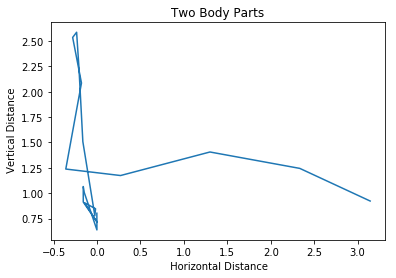
\includegraphics[width=0.75\columnwidth]{images/TwoBodyParts.png}\caption{Two body parts}\label{fig:partstaba}\end{subfigure}&
\begin{subfigure}{0.4\textwidth}\centering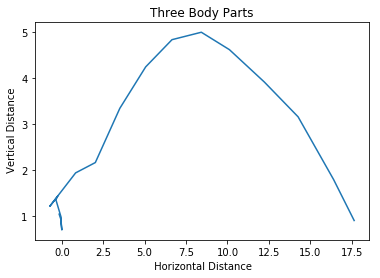
\includegraphics[width=0.75\columnwidth]{images/ThreeBodyParts.png}\caption{Three body parts}\label{fig:partstabb}\end{subfigure}\\
\newline
\begin{subfigure}{0.4\textwidth}\centering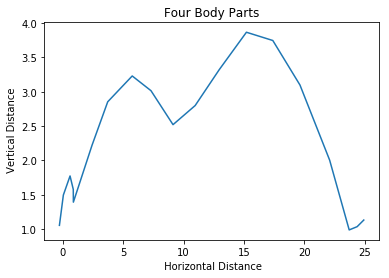
\includegraphics[width=0.75\columnwidth]{images/FourBodyParts.png}\caption{Four body parts}\label{fig:partstabc}\end{subfigure}&
\begin{subfigure}{0.4\textwidth}\centering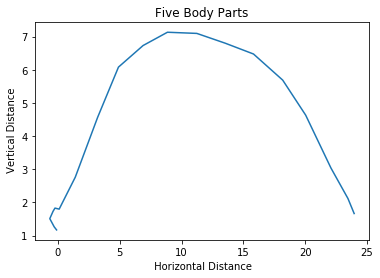
\includegraphics[width=0.75\columnwidth]{images/FiveBodyParts.png}\caption{Five body parts}\label{fig:partstabd}\end{subfigure}\\
\newline
\begin{subfigure}{0.4\textwidth}\centering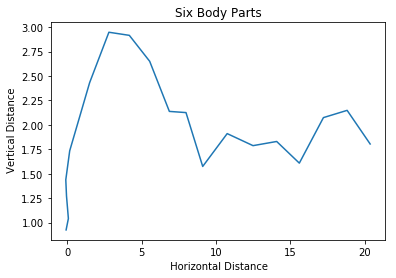
\includegraphics[width=0.75\columnwidth]{images/SixBodyParts.png}\caption{Six body parts}\label{fig:partstabe}\end{subfigure}&
\begin{subfigure}{0.4\textwidth}\centering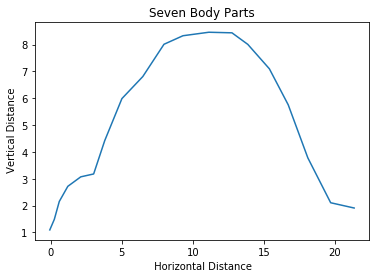
\includegraphics[width=0.75\columnwidth]{images/SevenBodyParts.png}\caption{Seven body parts}\label{fig:partstabf}\end{subfigure}\\
\end{tabular}
\caption{Path taken by caterpillars with different amounts of body parts.}
\label{tab:pathplotparts}
\end{table}
}

These are only single agent paths that are being shown here, but they were agents that were performing high-score or very close to it. Very noticeable is how the caterpillar with two bodyparts was entirely different than the rest of the group. Yet these data has to be observed with caution since it was only a single organism that is being displayed here. This merely shows that there is diversity, but this diversity also happens within a population of the same caterpillars. 

\newpage

And this data is more interesting and usable. When looking into the paths taken by multiple agents in a population of caterpillars with the same amount of body parts, we find that there are also multiple different paths being taken, that result in high scoring organisms. This it shows us that by the end of the 250 generations, there are multiple organisms in the population that can achieve peak performance scores using very different strategies(see Table \ref{tab:fourplotparts}, Figures \ref{fig:fourplotpartsa}, \ref{fig:fourplotpartsb}, \ref{fig:fourplotpartsc}, \ref{fig:fourplotpartsd}).

{\centering
\begin{table}[ht]
\begin{tabular}{cc}
\begin{subfigure}{0.4\textwidth}\centering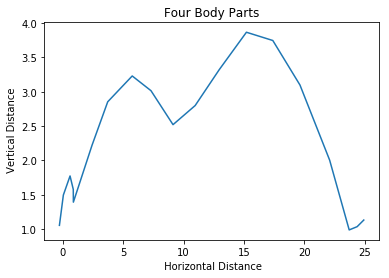
\includegraphics[width=0.75\columnwidth]{images/FourBodyParts.png}\caption{First Agent}\label{fig:fourplotpartsa}\end{subfigure}&
\begin{subfigure}{0.4\textwidth}\centering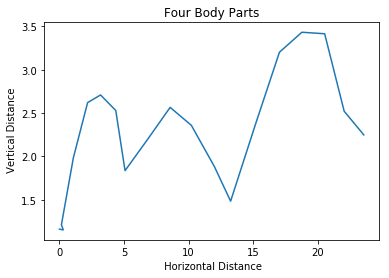
\includegraphics[width=0.75\columnwidth]{images/fourparts2.png}\caption{Second Agent}\label{fig:fourplotpartsb}\end{subfigure}\\
\newline
\begin{subfigure}{0.4\textwidth}\centering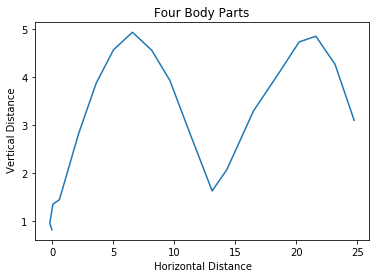
\includegraphics[width=0.75\columnwidth]{images/fourparts3.png}\caption{Third Agent}\label{fig:fourplotpartsc}\end{subfigure}&
\begin{subfigure}{0.4\textwidth}\centering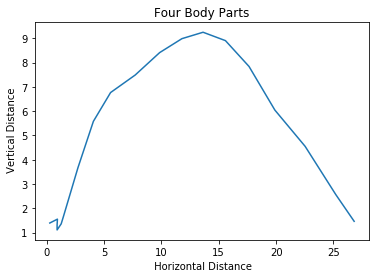
\includegraphics[width=0.75\columnwidth]{images/fourparts4.png}\caption{Fourth Agent}\label{fig:fourplotpartsd}\end{subfigure}\\
\end{tabular}
\caption{Four different examples of paths taken by caterpillars with four body parts}
\label{tab:fourplotparts}
\end{table}
}


\subsubsection{Bug during experiment} %OK?? Writing about this kind of stuff
After having run the experiment once I began plotting the data generated and soon had to find out that there was a bug in the code that falsified all the results the run had generated. I saw that the resetting function for the position did work in theory, but it did not reset the caterpillar centered, and it did not even spawn that way the first time around (see Figure \ref{fig:TwoPartsBugged}). That meant that something must be wrong fundamentally.
The more body parts the caterpillar had, which means the longer the caterpillar was, the further back it was in the opposite direction to scoring. This meant that longer caterpillars spent a considerable amount of time evolving with 0 score, since they had to move quite far to even gain minimal score improvements.
All other plots (except for Figure \ref{fig:TwoPartsBugged}) in this paper were created or replaced with the fixed and updated version.
\newpage
\begin{figure}[h!]
\centering
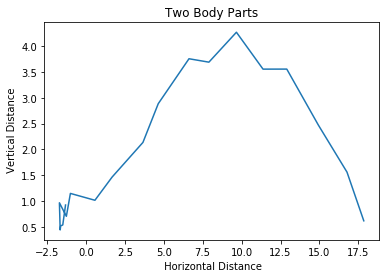
\includegraphics[width=0.75\textwidth,height=0.75\textheight,keepaspectratio]{images/2parts_bug.png}
\caption{A graph that shows the bug that occurred during the experiment in an earlier version.}
\label{fig:TwoPartsBugged}
\end{figure}

In this plot it is obvious how the caterpillar did not start at 0.
And to make things worse, this varied for caterpillars with different amounts of body parts, which falsifies the fitness function. 
To figure out by what factor the caterpillar was off, and to figure out which constants I could find in that I used different lengths and body parts and printed out the position for each joint. It soon became clear that the caterpillar was being spawned in a way in which the first joint was at position 0 and all the following joints and body parts were just overhanging back. To solve this I just had to move the caterpillar's position accordingly, which turned out to be 
\begin{lstlisting}[language=C++, label={lst:adjusteven}, caption=Adjusting Spawn Position Even]
physicsObject->getDof(3)->setPosition(-((numberOfOutputsPL->get(PT)/2)*((jointLengthPL->get(PT)+default_width)))+((jointLengthPL->get(PT)+default_width)*0.5));

\end{lstlisting}
for caterpillars with an even amount of body parts (see Listing \ref{lst:adjusteven}) and
\begin{lstlisting}[language=C++, label={lst:adjustuneven}, caption=Adjusting Spawn Position Uneven]
physicsObject->getDof(3)->setPosition(-((numberOfOutputsPL->get(PT)/2)*((jointLengthPL->get(PT)+default_width)))); 

\end{lstlisting}
for caterpillars with uneven numbers (see Listing \ref{lst:adjustuneven}).

With the new code in place, rerunning the whole experiment was the only option, since all the scores, and therefore the whole process of evolution was falsified. 

\subsubsection{Bodypart length}
The second experiment that was run using this method investigated the performance peak parameter for the length of bodyparts. The setup and structure under which this project was run is almost identical to the previous test. This time the parameter would run with the values 0.25, 0.5, 0.75, 1.0, 1.25, 1.5, 1.75, 2.0, 2.25, and 2.5 over 250 generations with a population of 100 and 50 replicates (see Figure \ref{fig:length_bars}). 

\begin{figure}[h!]
\centering
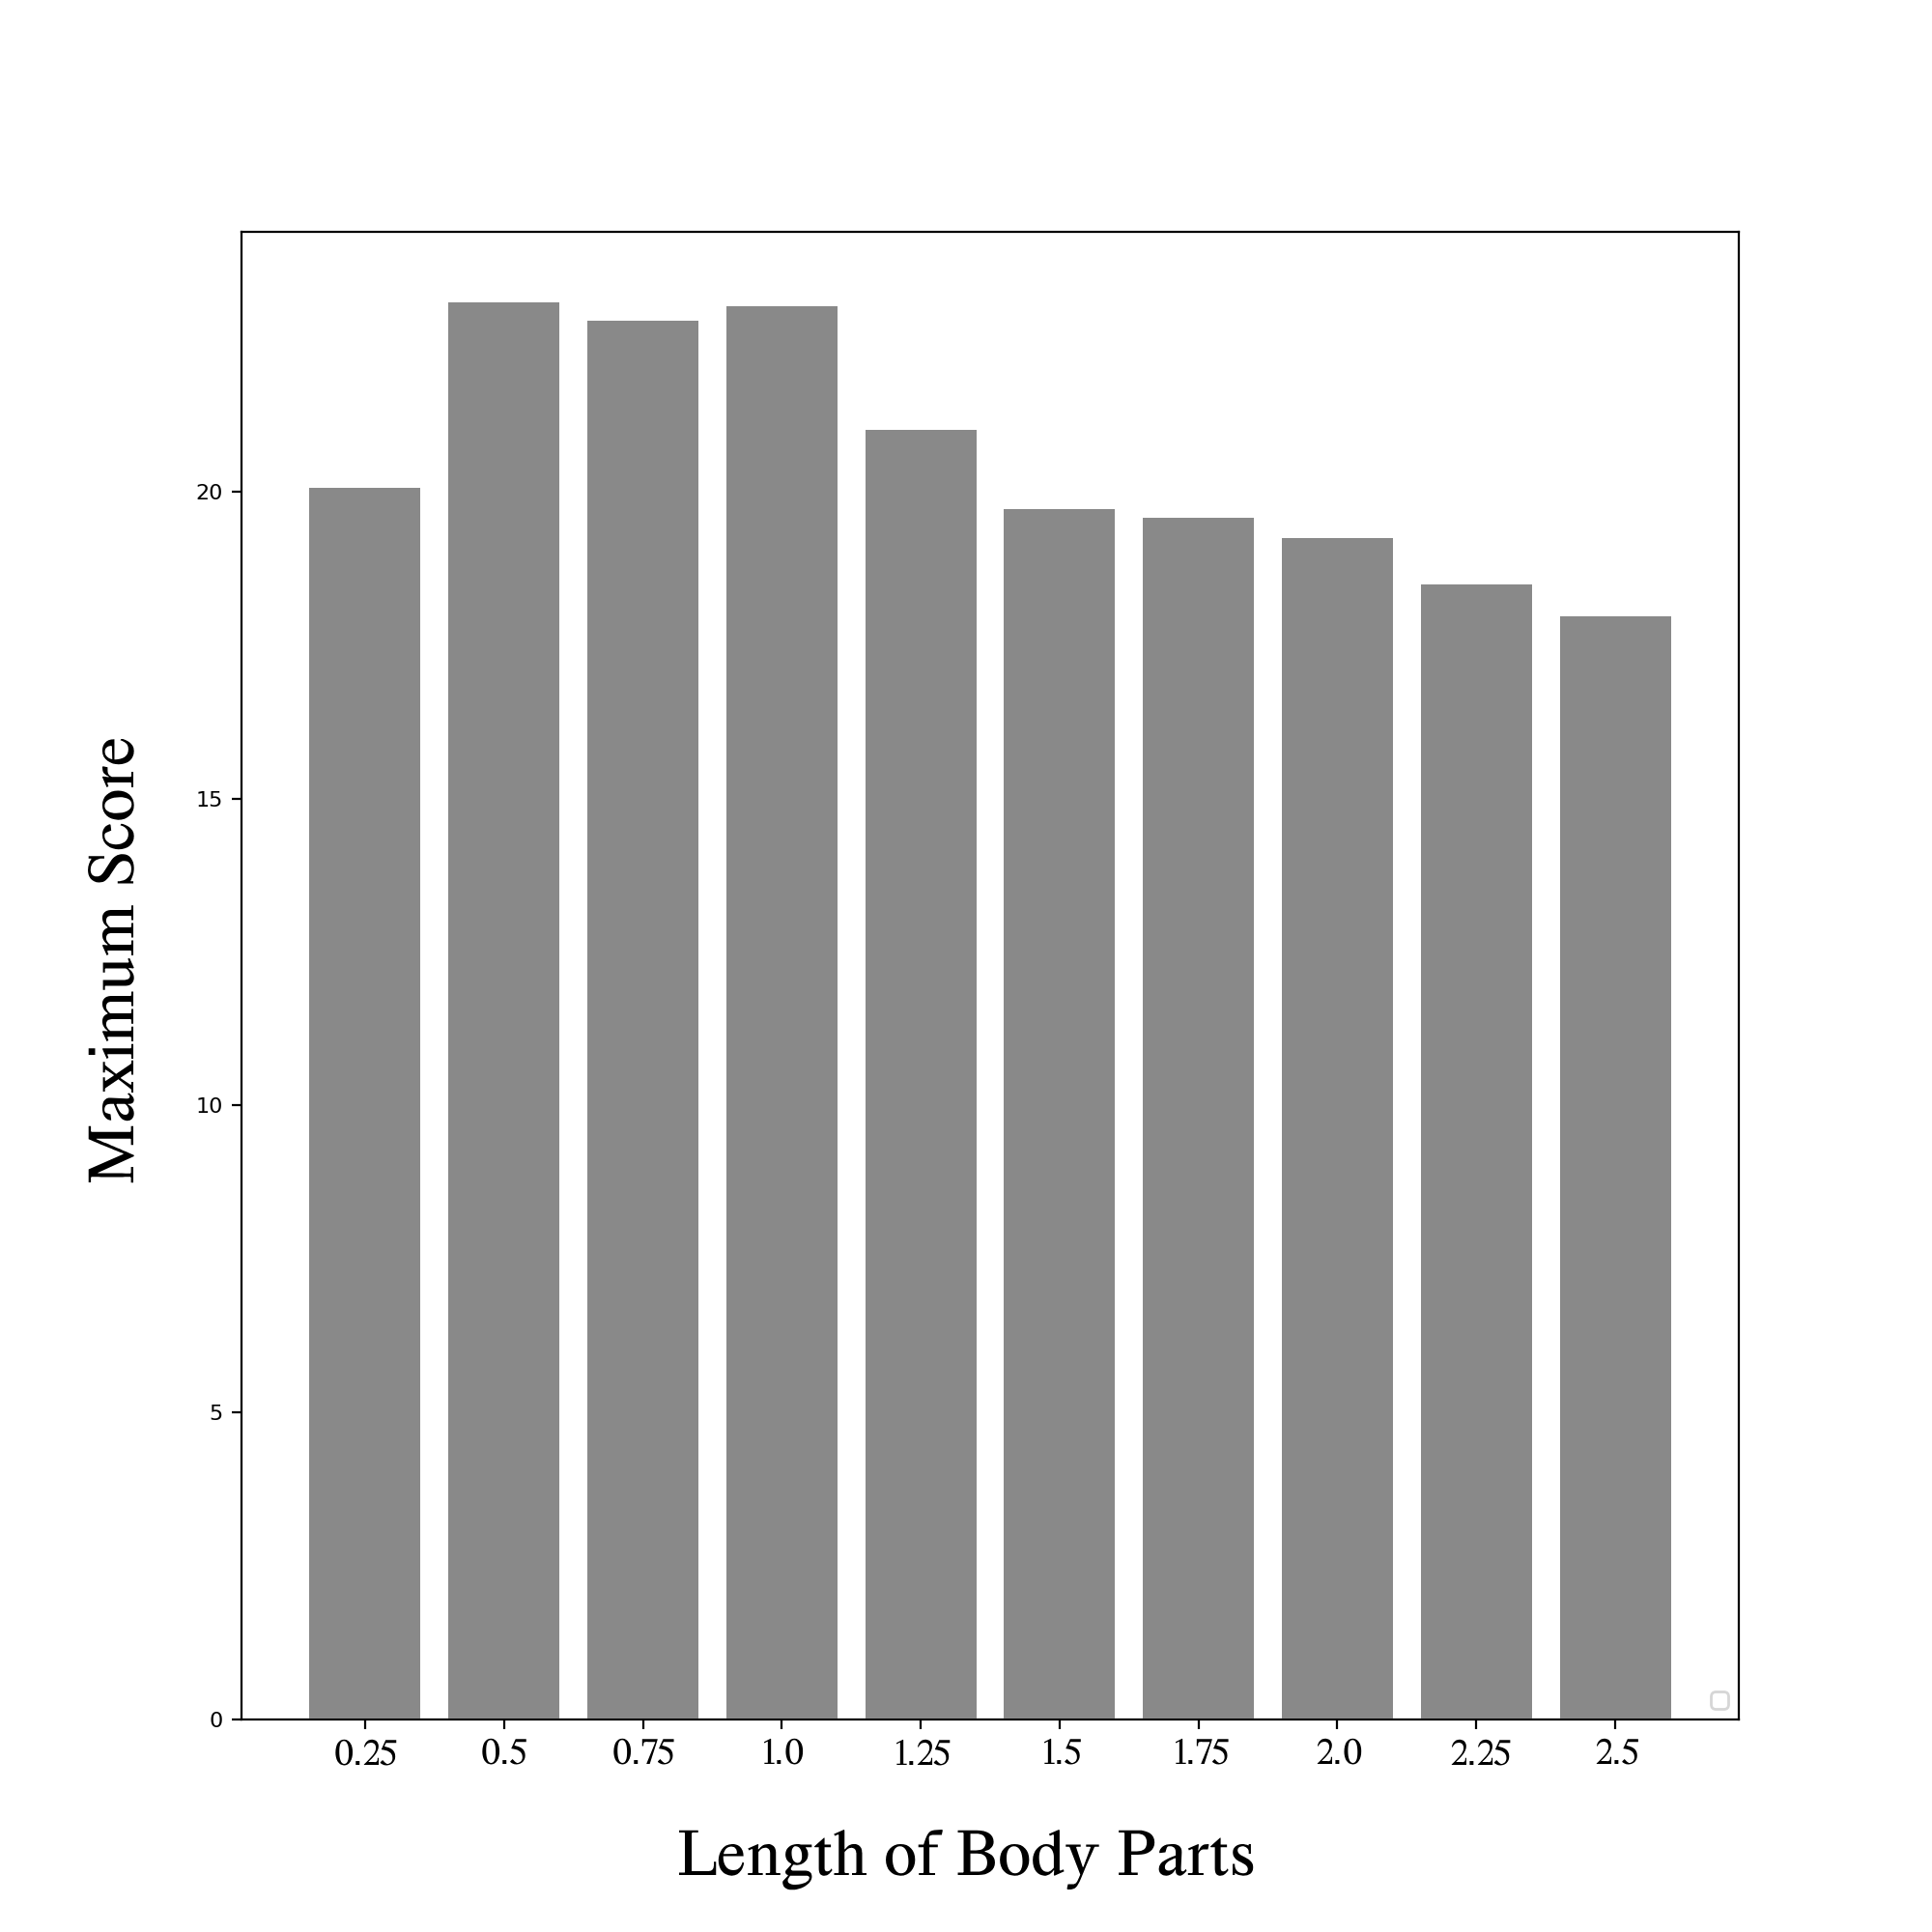
\includegraphics[width=0.75\textwidth,height=0.75\textheight,keepaspectratio]{images/length-bars.png}
\caption{Bar Plot displaying average score for each length of bodyparts}
\label{fig:length_bars}
\end{figure}

Besides the little dent that occurs at the length of 0.75 it seems from our experiment range that the peak is in the 0.5 to 1.0 range. With the values before and after being noticeably lower. This result is similar to the one we saw earlier when we looked at the plot for peak performance by caterpillars with different amounts of body parts. This makes it seem as though more complex bodies do not equal better score. It rather seems like as if there is a somewhat precise spot that, when hit, performs the best, with competitors of higher or lower complexity not reaching it's potential.  
We can again compare the path taken, represented by a single high scoring organism (see Table \ref{tab:pathplotlength}). Again, this is not providing much insight until we also compare a single populations paths (see Table \ref{tab:fourplotlength}).

\newpage

{\centering
\begin{table}[h!]
\begin{tabular}{cc}
\begin{subfigure}{0.4\textwidth}\centering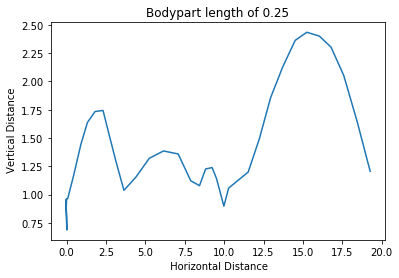
\includegraphics[width=0.75\columnwidth]{images/length_025.png}\caption{Bodypart Length of 0.25}\label{fig:lengthtaba}\end{subfigure}&
\begin{subfigure}{0.4\textwidth}\centering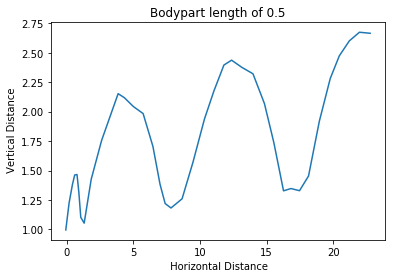
\includegraphics[width=0.75\columnwidth]{images/length_05.png}\caption{Bodypart Length of 0.5}\label{fig:lengthtabb}\end{subfigure}\\
\newline
\begin{subfigure}{0.4\textwidth}\centering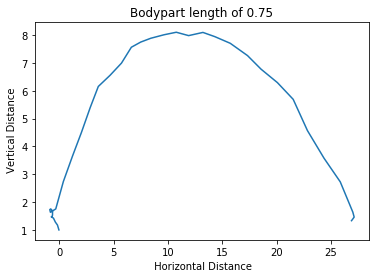
\includegraphics[width=0.75\columnwidth]{images/length_075_1.png}\caption{Bodypart Length of 0.75}\label{fig:lengthtabc}\end{subfigure}&
\begin{subfigure}{0.4\textwidth}\centering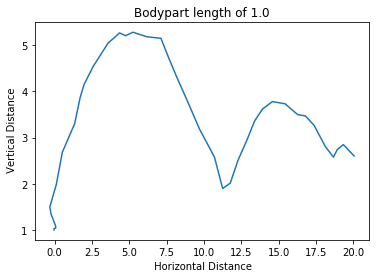
\includegraphics[width=0.75\columnwidth]{images/length_10.png}\caption{Bodypart Length of 1.0}\label{fig:lengthtabd}\end{subfigure}\\
\newline
\begin{subfigure}{0.4\textwidth}\centering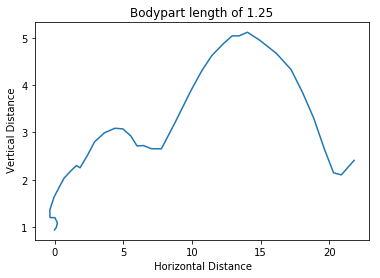
\includegraphics[width=0.75\columnwidth]{images/length_125.png}\caption{Bodypart Length of 1.25}\label{fig:lengthtabe}\end{subfigure}&
\begin{subfigure}{0.4\textwidth}\centering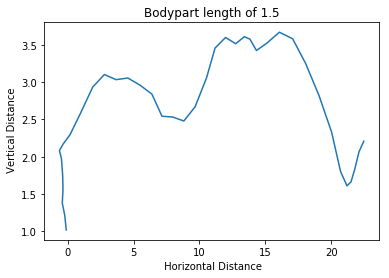
\includegraphics[width=0.75\columnwidth]{images/length_15.png}\caption{Bodypart Length of 1.5}\label{fig:lengthtabf}\end{subfigure}\\
\newline
\begin{subfigure}{0.4\textwidth}\centering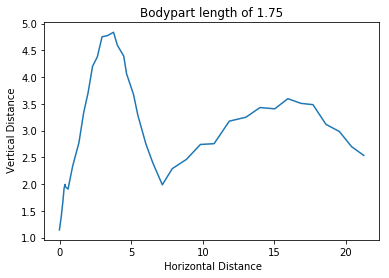
\includegraphics[width=0.75\columnwidth]{images/length_175.png}\caption{Bodypart Length of 1.75}\label{fig:lengthtabg}\end{subfigure}&
\begin{subfigure}{0.4\textwidth}\centering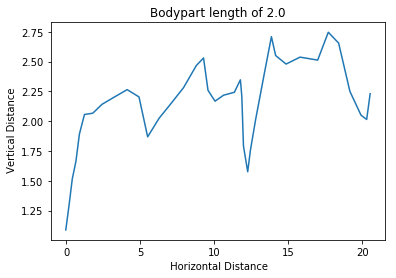
\includegraphics[width=0.75\columnwidth]{images/length_20.png}\caption{Bodypart Length of 2.0}\label{fig:lengthtabh}\end{subfigure}\\
\newline
\begin{subfigure}{0.4\textwidth}\centering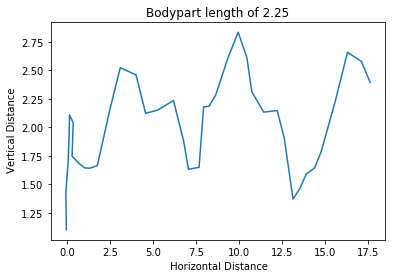
\includegraphics[width=0.75\columnwidth]{images/length_225.png}\caption{Bodypart Length of 2.25}\label{fig:lengthtabi}\end{subfigure}&
\begin{subfigure}{0.4\textwidth}\centering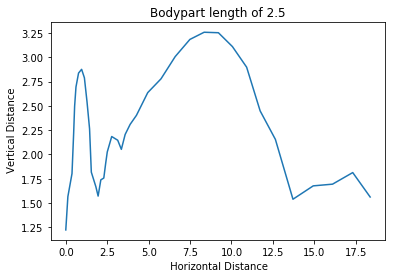
\includegraphics[width=0.75\columnwidth]{images/length_25.png}\caption{Bodypart Length of 2.5}\label{fig:lengthtabj}\end{subfigure}\\
\end{tabular}
\caption{Path taken by caterpillars with different body part lengths}
\label{tab:pathplotlength}
\end{table}
}

\newpage

{\centering
\begin{table}[h!]
\begin{tabular}{cc}
\begin{subfigure}{0.4\textwidth}\centering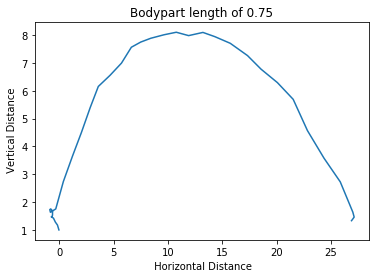
\includegraphics[width=0.75\columnwidth]{images/length_075_1.png}\caption{First Agent}\label{fig:fourplotlengtha}\end{subfigure}&
\begin{subfigure}{0.4\textwidth}\centering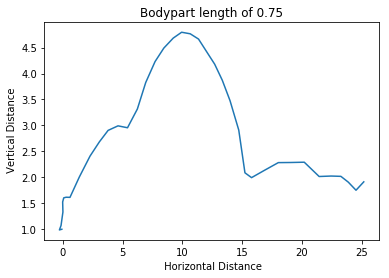
\includegraphics[width=0.75\columnwidth]{images/length_075_2.png}\caption{Second Agent}\label{fig:fourplotlengthb}\end{subfigure}\\
\newline
\begin{subfigure}{0.4\textwidth}\centering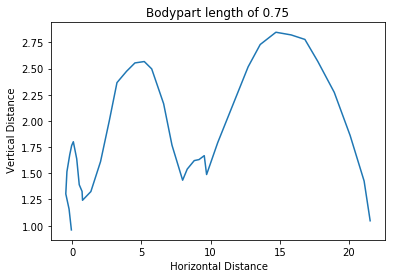
\includegraphics[width=0.75\columnwidth]{images/length_075_3.png}\caption{Third Agent}\label{fig:fourplotlengthc}\end{subfigure}&
\begin{subfigure}{0.4\textwidth}\centering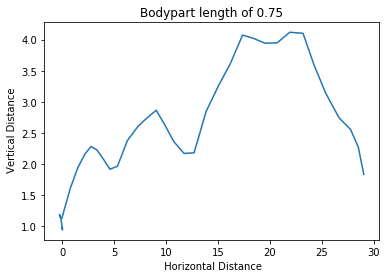
\includegraphics[width=0.75\columnwidth]{images/length_075_4.png}\caption{Fourth Agent}\label{fig:fourplotlengthd}\end{subfigure}\\
\end{tabular}
\caption{Four different examples of paths taken by caterpillars with a body part length of 0.75}
\label{tab:fourplotlength}
\end{table}
}

Again the observation can be made that multiple organisms are still within the population that seem to have found a way to reach peak performance or very close to it. Since mutation was enabled, running the experiment longer would not resolve this ``issue'', since fixation would never be reached. 

%Bevor HPCC immer noch alles so ein wenig proof of concept. Man lernt aus fehlern und so.
%Ihnalt nicht so wichtig -> funktioniert!!
%Alles klappt, yeah!


\subsubsection{HPCC} \label{sssec:hpcc}
One issue that held back further experiments in the later stages of development and research was the infrastructure and the circumstances under which we had to work due to my status at MSU. Neither did I have access to the High Performance Computers, nor did they have the software needed on there, which meant that experiments had to run for up to 12 days, which made for a very slow cycle in which I could obtain data and analyse it to run follow ups. After completing the initial 12 day experiment, and still not having heard back from the HPCC administrators, the best alternative was to split the experiment in up to 8 smaller bits that made up the original one to make use of all 8 cores available to me and therefore cut down the run-time by a factor of 8. This still took longer than it should have, but was the best available option in the given scenario.
\newpage
\section{Discussion}
Looking back on where we were in September of 2018 and comparing the goals we had set back then to the product we have developed since then most of our demands were met, on way or another. Not everything is encoded the way we had first thought of handling it in the beginning, but some components and features have been adjusted to DART, modified in a way that was more suitable to the experiments we ran, were more performant, made more sense in the scope of a implementation and proof of concept state or just simply were more appealing to me more personally. First we had envisioned to create a large cube made up of many smaller softbody cubes which could then inflate and deflate on the brains command, which would then move the whole structure, with morphology possibly taking over the size of the cube, similar to how Jeff Clune did it in his paper~\cite{cheney2014unshackling}.


\begin{figure}[h!]
\centering
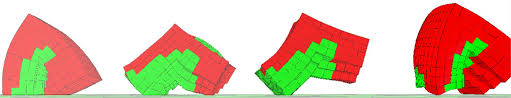
\includegraphics[width=0.75\textwidth,height=0.75\textheight,keepaspectratio]{images/clunecube.jpeg}
\caption{Clune's morphology cube's movement displayed by 4 stills over time.~\cite{cheney2014unshackling}}
\label{fig:clune}
\end{figure}


But after having spent a good amount of time on godot and softbodies we decided to only investigate if softbodies theoretically work in dart before moving on to actual implementation soon after, using rigid bodies and muscles instead. 
The goal of the world and task the agent performs was left open for me to decide, which I gladly accepted. I went straight for movement performance, since that has fascinated me for a long time already. But that goal, the fitness, is very easily modifiable, without having to change too much code.
The main goal, which was having a physics environment implement within Hintze Lab's own framework MABE was achieved well within time with the proof of concept ``Ball Pushing'' world about half way through my stay. This allowed us to dive deeper into the matter and create more complex scenarios and challenges (caterpillar experiments) and even open up the door for me to research a bit towards complexity. Going beyond just coding to make things work, and into actually applying the code to look into how body complexity affects the complexity of movement.


Overall, the goals have been met, even if the way to get there may differ from the original blueprint. 
\newpage
\section{Outlook}
This feature had been wished for and planned in Hintze Lab for a long time already and had already been attempted in unity and with the bullet physics engine, with little success though, due to limited time and limitation by the engines. 
\newline Now that MABE allows for complex evolution to take place in the way of three dimensional physics, a lot of new research is possible, morphology being one of them. Using genomes and letting them control the body structure and assembly and letting it coevolve with the brain which is a field that has not gotten a lot of attention yet.
\newline This should also help to spread MABE out more among researchers all over the nation and even internationally, with the software package now allowing to write complex worlds, be it morphology or other complex environments outside of morphology, with physics already in place.
\newline MABE, with the implementation of 3D physics, now offers the ability for a lot of new and exciting research that was not possible before. 



\backmatter

\bibliographystyle{plain}
\bibliography{references}


%----------------------------------------------------------------------------------------------------
\newpage
\chapter{Attachments}
\section{CD Content}
\begin{itemize}
  \item Code (The caterpillar code written by me can be found in MabePhysics/World/PhysicsWorld)
  \item Thesis as PDF file
  \item Sources
\end{itemize}



\newpage
\thispagestyle{empty}

% Bitte hier keine Änderungen vornehmen, sondern vollständig handschriftlich ausfüllen

% \noindent  {\Large \textbf{Erklärung}}\\
\noindent  {\Large \textbf{Declaration}}\\

\vspace*{2cm}


\noindent
I hereby declare and confirm that this thesis is entirely the result of my own original work. Where other sources of information have been used, they have been indicated as such and properly acknowledged. I further declare that this or similar work has not been submitted for credit elsewhere.
\vspace{2cm}

\noindent
Kempten, March 12th 2019 
\hspace*{2cm}%
\dotfill\\
\hspace*{8.5cm}%
\textit{David Richter}

\vspace*{5cm}

\noindent  {\Large \textbf{Authorization}}\\

\vspace*{2cm}

\noindent
I hereby authorize the university for applied sciences Kempten to publish the abstract of my work on e.g. printed media or a website.
\vspace{2cm}

\noindent
Kempten, March 12th 2019 
\hspace*{2cm}%
\dotfill\\
\hspace*{8.5cm}%
\textit{David Richter}

%------------------------------------------------------------------------------------------

\newpage
\shipout\null

\end{document}

%Explain code in more detail like for example the reset function